% Báo cáo kỹ thuật WikiPulse -- bản cập nhật liên tục của cả nhóm.
% Định dạng theo mẫu báo cáo của Trường CNTT&TT, ĐHBK Hà Nội (lớp report 12pt, lề 2,5 cm, giãn dòng 1,5,
% phông Latin Modern, tài liệu tham khảo BibTeX kiểu plain). Quy ước cập nhật: xem chương đầu và README.md.
% Biên dịch: latexmk -xelatex main.tex  (hoặc xelatex main -> bibtex main -> xelatex main -> xelatex main)
\documentclass[12pt,a4paper]{report}

% ============================================================================
\usepackage{fontspec}               % XeLaTeX: phông Latin Modern (giống Computer Modern, đủ dấu tiếng Việt)
\usepackage[vietnamese]{babel}
\usepackage{amsmath,amssymb,amsfonts}
\usepackage{graphicx}
\usepackage{booktabs}
\usepackage{longtable}
\usepackage{array}
\usepackage{tabularx}
\usepackage{multirow}
\usepackage{algorithm}
\usepackage[noend]{algpseudocode}
\usepackage{listings}               % chỉ dùng bộ đếm và tên "Đoạn mã"; khối mã viết bằng fancyvrb (đúng chữ có dấu)
\usepackage{fancyvrb}
\usepackage[table]{xcolor}
\usepackage{hyperref}
\usepackage{geometry}
\usepackage{setspace}
\usepackage{caption}
\usepackage{subcaption}
\usepackage{float}
\usepackage{enumitem}
\usepackage{url}
\usepackage{tcolorbox}
\usepackage{tikz}
\usetikzlibrary{arrows.meta,positioning,shapes.geometric,shapes.misc,shapes.multipart,calc,fit,backgrounds}
\usepackage{pgf-umlsd}            % biểu đồ tuần tự UML
\usepackage{pgfplots}
\pgfplotsset{compat=1.18}

\geometry{margin=2.5cm}
\onehalfspacing
\graphicspath{{hinh/}}
\setcounter{tocdepth}{2}
\hypersetup{hidelinks}
\setlist{itemsep=1pt,topsep=3pt}
\emergencystretch=3em          % tránh tràn lề khi dòng có tên mã dài không ngắt được

\newcommand{\enquote}[1]{“#1”}
\newcommand{\code}[1]{\texttt{#1}}
\newcommand{\chualam}{\par\noindent\textit{(Dự kiến, chưa thực hiện.)}\par}
% Ghi chú nhỏ dưới một mục đã viết nhưng còn sửa ở các tuần sau
\newcommand{\dukiensua}[1]{\par\noindent{\footnotesize\itshape\color{black!60}Ghi chú: #1}\par}
% Thông tin còn thiếu, cần bổ sung
\newcommand{\canbosung}[1]{{\color{red}[#1]}}

\renewcommand{\lstlistingname}{Đoạn mã}

% Từ khóa giả mã giữ tiếng Anh chuẩn (Input, Output, for, if, return...); chỉ phần mô tả viết tiếng Việt
\algrenewcommand\algorithmicrequire{\textbf{Input:}}
\algrenewcommand\algorithmicensure{\textbf{Output:}}
\algnewcommand\algorithmicand{\textbf{and}}
\algnewcommand\AlgAnd{\algorithmicand}
\floatname{algorithm}{Thuật toán}

% Màu dùng trong sơ đồ
\definecolor{wpblue}{RGB}{18,92,173}
\definecolor{wpgreen}{RGB}{46,140,87}
\definecolor{wpamber}{RGB}{214,140,20}
\definecolor{wpred}{RGB}{190,50,50}
\definecolor{wpgray}{RGB}{110,116,128}
\definecolor{lightblue}{RGB}{228,239,252}
\definecolor{lightgreen}{RGB}{224,244,232}
\definecolor{lightamber}{RGB}{255,241,214}
\definecolor{lightred}{RGB}{252,226,226}
\definecolor{lightgray}{RGB}{242,243,245}

% Hộp ghi chú: khung mảnh, nền xám nhạt, hợp văn phong báo cáo
\newtcolorbox{ghichu}[1]{colback=lightgray,colframe=black!55,boxrule=0.4pt,arc=0pt,
  fonttitle=\bfseries,coltitle=black,colbacktitle=black!10,title=#1}

\tikzset{
  box/.style={draw=wpblue,fill=lightblue,rounded corners=3pt,align=center,font=\small\sffamily,
              minimum height=9mm,inner sep=4pt,text width=#1},
  box/.default=28mm,
  gbox/.style={box=#1,draw=wpgreen,fill=lightgreen},
  gbox/.default=28mm,
  abox/.style={box=#1,draw=wpamber,fill=lightamber},
  abox/.default=28mm,
  rbox/.style={box=#1,draw=wpred,fill=lightred},
  rbox/.default=28mm,
  db/.style={cylinder,shape border rotate=90,aspect=0.18,draw=wpblue,fill=lightblue,
             align=center,font=\small\sffamily,minimum height=13mm,text width=24mm},
  dec/.style={diamond,aspect=2.2,draw=wpamber,fill=lightamber,align=center,font=\small\sffamily,inner sep=1pt},
  arr/.style={-{Stealth[length=2.6mm]},thick,color=wpgray},
  lab/.style={font=\scriptsize\sffamily,color=wpgray,fill=white,inner sep=1pt},
  uc/.style={ellipse,draw=wpblue,fill=lightblue,align=center,font=\footnotesize\sffamily,
             minimum width=40mm,minimum height=9mm,inner sep=1pt},
  actor/.pic={\draw[thick] (0,0.42) circle (0.16);
              \draw[thick] (0,0.26) -- (0,-0.12) (-0.28,0.14) -- (0.28,0.14) (0,-0.12) -- (-0.2,-0.46) (0,-0.12) -- (0.2,-0.46);},
  % --- UML: biểu đồ hoạt động ---
  start/.style={circle,fill=black,minimum size=3.2mm,inner sep=0},
  stop/.style={circle,draw=black,thick,fill=white,minimum size=4.4mm,inner sep=0,
               path picture={\fill[black] (path picture bounding box.center) circle (1.25mm);}},
  act/.style={rectangle,rounded corners=2.5mm,draw=black,fill=lightblue,align=center,font=\footnotesize\sffamily,
              minimum height=8mm,inner sep=3pt,text width=#1},
  act/.default=40mm,
  dnode/.style={diamond,draw=black,fill=white,minimum size=6.5mm,inner sep=0},
  flow/.style={-{Stealth[length=2.2mm]},thick},
  guard/.style={font=\scriptsize\sffamily,fill=white,inner sep=1pt},
  % --- UML: biểu đồ trạng thái ---
  state/.style={rectangle,rounded corners=3mm,draw=black,fill=lightblue,align=center,font=\footnotesize\sffamily,
                minimum height=9mm,minimum width=24mm,inner sep=3pt},
  % --- UML: biểu đồ gói, triển khai ---
  pkg/.style={rectangle,draw=black,fill=lightblue,align=center,font=\footnotesize\sffamily,minimum width=24mm,
              minimum height=9mm,inner sep=2pt,
              append after command={\pgfextra{\draw[fill=lightblue] (\tikzlastnode.north west) rectangle ++(8mm,2.4mm);}}},
  dep/.style={-{Straight Barb[length=2mm]},dashed,thick},
  udnode/.style={rectangle,draw=black,fill=lightblue,align=center,font=\footnotesize\sffamily,inner sep=4pt,
                 append after command={\pgfextra{\draw (\tikzlastnode.north west) -- ++(3mm,3mm)
                   -- ($(\tikzlastnode.north east)+(3mm,3mm)$) -- ($(\tikzlastnode.south east)+(3mm,3mm)$)
                   -- (\tikzlastnode.south east) ($(\tikzlastnode.north east)+(3mm,3mm)$) -- (\tikzlastnode.north east);}}},
  % --- sơ đồ CSDL (sinh bởi tools/erd.py) ---
  erd/.style={rectangle split,rectangle split parts=2,draw=black,anchor=north west,font=\scriptsize\sffamily,
              rectangle split part fill={lightblue,white},inner sep=2pt},
  erdstub/.style={draw=black,dashed,anchor=north west,font=\scriptsize\sffamily,inner sep=4pt,fill=lightgray},
  erdline/.style={thick},
  erdmult/.style={font=\scriptsize\sffamily,fill=white,inner sep=1pt},
  erdfk/.style={font=\tiny\sffamily,color=wpgray,sloped,above,inner sep=1pt},
}

% ============================================================================
% DOCUMENT BEGIN
% ============================================================================

% ============================================================================
% DOCUMENT BEGIN
% ============================================================================
\begin{document}


% ============================================================================
% TRANG BÌA (theo mẫu báo cáo của Trường CNTT&TT)
% ============================================================================
\begin{titlepage}
\begin{center}

\textsc{\large \textbf{ĐẠI HỌC BÁCH KHOA HÀ NỘI}}\\[0.5cm]

{\Large TRƯỜNG CÔNG NGHỆ THÔNG TIN VÀ TRUYỀN THÔNG \\[0.6cm]}


\includegraphics[scale=0.11]{logo-soict-hust-1.png}\\[0.6cm]
\textsc{\Large Học phần: \textbf{IT4043E}}\\[0.4cm]

\rule{\linewidth}{0.7mm} \\[0.4cm]
{\huge \bfseries WikiPulse\\[0.3cm]}
{\Large \bfseries Phân tích xu hướng chỉnh sửa đáng ngờ \\ theo thời gian thực trên Wikipedia\\[0.3cm]}
\rule{\linewidth}{0.7mm} \\[0.6cm]

{\large \textbf{Giảng viên hướng dẫn:}}\\[0.3cm]
\begin{tabular}{l}
\large Trần Việt Trung \\[0.4cm]
\end{tabular}

{\large \textbf{Nhóm sinh viên thực hiện:}}\\[0.3cm]
\begin{tabular}{ll}
\large Trần Quang Trọng & \large 20235565 \\
\large Lê Nguyễn Phước Thành & \large 20235561 \\
\large Nguyễn Ngọc Linh & \large 20235520 \\
\large Hoàng Văn Nhân & \large 20235542 \\
\large Nguyễn Đức Mạnh & \large 20235525 \\
\end{tabular}

\end{center}
\end{titlepage}
\setstretch{1.5}

\pagenumbering{roman}

\tableofcontents
\newpage
\chapter*{Danh mục thuật ngữ và viết tắt}
\addcontentsline{toc}{chapter}{Danh mục thuật ngữ và viết tắt}
\small
\begin{longtable}{@{}p{0.32\linewidth}p{0.63\linewidth}@{}}
\toprule
\textbf{Thuật ngữ} & \textbf{Giải thích} \\
\midrule
\endfirsthead
\toprule
\textbf{Thuật ngữ} & \textbf{Giải thích} \\
\midrule
\endhead
ACK (acknowledgement) & Xác nhận kết quả một lần gửi; Kafka ACK không tự chứng minh exactly-once. \\
Aggregation & Phép tổng hợp nhiều event thành kết quả theo nhóm. \\
Allowlist & Danh sách các giá trị được phép xử lý trong phạm vi cấu hình. \\
Analytics & Phân tích dữ liệu để tính đặc trưng hoặc kết quả nghiệp vụ. \\
Analytics sink & Nơi nhận kết quả analytics, chẳng hạn Parquet hoặc Cassandra theo cấu hình. \\
Anonymity & Trạng thái không thể xác định danh tính; pseudonymization không tự bảo đảm điều này. \\
API (application programming interface) & Giao diện để các chương trình yêu cầu và nhận dữ liệu. \\
API request & Một yêu cầu tới API; một request có thể cần nhiều query hoặc partition. \\
Append mode & Output mode chỉ ghi thêm dòng mới; với aggregation theo event time, watermark có thể ảnh hưởng thời điểm xuất. \\
Backoff & Cách tăng thời gian chờ giữa các lần thử lại sau lỗi. \\
Batch / micro-batch & Một nhóm dữ liệu được xử lý cùng nhau; micro-batch là nhóm nhỏ lấy từ stream. \\
Broker & Tiến trình Kafka lưu và phục vụ dữ liệu topic. \\
Bronze / Silver / Gold & Các tầng lưu raw data, dữ liệu được chuẩn hóa và kết quả tổng hợp đã chốt. \\
Canary event & Sự kiện kiểm tra của Wikimedia; được giữ trong Bronze raw, không đưa vào business metrics. \\
Cassandra & Cơ sở dữ liệu phân tán, dùng để phục vụ truy vấn theo khóa. \\
Checkpoint (project) & Mốc nghiệm thu của nhóm, ví dụ CP0--CP4; khác Spark checkpoint. \\
Checkpoint (Spark) & Dữ liệu Spark lưu về offset và state để phục hồi một query. \\
Clean clone & Bản sao repo mới lấy từ commit xác định, không chứa thay đổi working tree chưa commit. \\
Clustering key & Phần khóa xác định thứ tự các dòng trong một Cassandra partition. \\
Collector & Chương trình nhận event từ nguồn rồi gửi tới Kafka. \\
Consumer / producer & Chương trình đọc / ghi dữ liệu vào một hệ thống như Kafka. \\
Container / image & Môi trường chạy được cách ly / bản đóng gói dùng để tạo container. \\
Contract & Quy ước chung về dữ liệu và hành vi giữa producer và consumer. \\
Cursor & Vị trí trong stream dùng để yêu cầu tiếp tục đọc khi kết nối lại. \\
Dashboard & Giao diện tổng hợp dữ liệu cho người dùng. \\
Dead-letter queue (DLQ) & Nơi dự kiến nhận bản ghi lỗi; topic được tạo nhưng sink Kafka DLQ còn chờ nhóm quyết định. \\
Deduplication & Loại bản ghi trùng theo khóa và phạm vi state được cấu hình; không bảo đảm vô hạn. \\
Docker Compose / profile & Công cụ cấu hình các dịch vụ container / nhóm dịch vụ được bật theo nhu cầu. \\
Duplicate & Bản ghi lặp lại một event logic; deduplication xử lý theo quy tắc và phạm vi state. \\
End-to-end (E2E) & Đánh giá một luồng qua các thành phần từ đầu vào tới đầu ra được xác định. \\
Endpoint & Địa chỉ API nhận một loại request cụ thể. \\
Envelope & Nội dung event và metadata được chuẩn bị trước khi gửi Kafka. \\
Event / event ID & Sự kiện nguồn / định danh dùng để phân biệt sự kiện. \\
Event time / processing time & Thời điểm nguồn gắn cho sự kiện / thời điểm hệ thống xử lý sự kiện. \\
Exactly-once & Bảo đảm mỗi tác động logic chỉ xảy ra một lần trong phạm vi được xác định; dự án không cam kết end-to-end. \\
FastAPI / Streamlit & Framework Python cung cấp API / công cụ xây dashboard. \\
Fixture / golden result & Dữ liệu kiểm thử cố định / kết quả kỳ vọng được chuẩn bị độc lập để đối chiếu. \\
Hadoop Distributed File System (HDFS) & Hệ thống file phân tán gồm NameNode quản lý metadata và DataNode lưu block. \\
Hash & Giá trị tạo từ dữ liệu đầu vào qua hàm băm. \\
Header & Trường thông tin đi kèm request hoặc response, chẳng hạn Last-Event-ID. \\
Heuristic & Quy tắc ước lượng dựa trên dấu hiệu, không bảo đảm kết luận đúng cho mọi trường hợp. \\
High availability & Khả năng duy trì dịch vụ khi một thành phần gặp sự cố. \\
HTTP / status code & Giao thức truyền dữ liệu web / mã cho biết kết quả yêu cầu HTTP. \\
Ingestion & Bước nhận dữ liệu từ nguồn và đưa vào hệ thống. \\
Java Virtual Machine (JVM) & Môi trường thực thi chương trình Java, được Spark sử dụng. \\
JSON / JSON Lines (JSONL) & Định dạng dữ liệu văn bản / cách lưu thường gồm một giá trị JSON trên mỗi dòng. \\
Kafka & Hệ thống lưu và truyền stream theo topic và partition. \\
Kafka key / offset & Key giúp định tuyến event tới partition / vị trí của bản ghi trong partition đó. \\
Keyspace & Không gian tên chứa các bảng Cassandra. \\
Last-Event-ID & HTTP header mang SSE ID của vị trí client yêu cầu tiếp tục khi kết nối lại. \\
Late event & Sự kiện đến sau các sự kiện có event time lớn hơn; cách xử lý phụ thuộc watermark và query. \\
Latency & Khoảng thời gian từ mốc bắt đầu tới mốc kết thúc được xác định của phép đo. \\
LIVE / REPLAY & Chế độ nhận stream thật / phát lại dữ liệu đã lưu. \\
Metadata & Thông tin mô tả dữ liệu, chẳng hạn nguồn hoặc thời điểm ingestion. \\
Node & Một máy hoặc tiến trình tham gia hệ thống phân tán. \\
Normalization & Bước chuẩn hóa dữ liệu về định dạng và ý nghĩa thống nhất. \\
Offset / end offset & Vị trí trong Kafka partition / vị trí tiếp theo ở cuối partition. \\
Original timing & Chế độ replay tính khoảng chờ từ chênh lệch event time của dữ liệu nguồn. \\
Output mode & Cách Spark xuất kết quả của streaming query, ví dụ update hoặc append. \\
Parquet & Định dạng file lưu theo cột, dùng cho các tầng dữ liệu phân tích. \\
Partition & Phần dữ liệu được chia theo ngữ cảnh: Kafka partition, Cassandra partition hoặc thư mục partition của file. \\
Partition key & Phần khóa xác định Cassandra partition để truy vấn. \\
Payload / raw data & Nội dung bản ghi / dữ liệu nguồn chưa được xử lý nghiệp vụ. \\
Pipeline & Chuỗi các bước đưa dữ liệu từ đầu vào qua xử lý tới đầu ra. \\
Polling & Kiểm tra trạng thái định kỳ cho đến khi đạt điều kiện hoặc hết thời hạn. \\
Process & Một tiến trình đang chạy; bộ nhớ cursor LIVE hiện gắn với process đó. \\
Provisional / finalized & Kết quả tạm tính có thể thay đổi / kết quả cửa sổ đã được chốt theo tiến độ event time. \\
Pseudonymization / salt & Thay định danh bằng mã giả / giá trị bổ sung khi băm; không đảm bảo ẩn danh tuyệt đối. \\
Query & Tác vụ hoặc truy vấn xử lý dữ liệu; Spark streaming query chạy liên tục. \\
Raw topic & Kafka topic nhận event ở đầu vào trước các bước xử lý downstream. \\
Readiness / health check & Điều kiện sẵn sàng nhận việc / phép kiểm trạng thái một thành phần. \\
Reconnect / resume / retry & Kết nối lại / yêu cầu đọc tiếp từ vị trí / thử lại thao tác sau lỗi. \\
Regression test & Test kiểm tra thay đổi không làm hỏng hành vi đã được hỗ trợ. \\
Restart & Dừng và khởi động lại một process hoặc dịch vụ. \\
Risk score / trend score & Điểm ưu tiên xem xét chỉnh sửa / điểm phản ánh mức độ hoạt động của trang theo công thức cấu hình. \\
Schema & Mô tả cấu trúc và kiểu dữ liệu của bản ghi hoặc bảng. \\
Scoring / rule & Cách tính điểm theo các quy tắc và cấu hình đã xác định. \\
Server-Sent Events (SSE) & Cách server gửi luồng sự kiện qua kết nối HTTP. \\
Serving & Phần lưu trữ và cung cấp dữ liệu cho các ứng dụng truy vấn. \\
Sink & Đích nhận kết quả của query, như Parquet hoặc Cassandra. \\
Snapshot & Bản chụp trạng thái dữ liệu hoặc mã tại một thời điểm. \\
State & Dữ liệu trung gian mà một query lưu để xử lý các batch tiếp theo. \\
Stream & Chuỗi sự kiện đến liên tục theo thời gian. \\
Structured Streaming & Thư viện Spark xử lý stream dựa trên query và state. \\
Time to live (TTL) & Thời gian lưu tối đa trước khi bản ghi hết hạn theo cấu hình. \\
Timestamp & Giá trị biểu diễn một thời điểm. \\
Topic & Kênh Kafka lưu bản ghi và được chia thành các partition. \\
Trigger & Cấu hình điều khiển thời điểm Spark bắt đầu xử lý batch. \\
Update mode & Output mode xuất kết quả của những nhóm có thay đổi trong batch. \\
Upsert & Ghi theo khóa: thêm nếu chưa có hoặc cập nhật nếu đã có. \\
Use case & Tình huống mô tả tương tác của tác nhân với hệ thống. \\
User hash & Mã băm có salt tạo từ user để thay định danh trực tiếp trong Silver. \\
Validation & Bước kiểm tra dữ liệu theo điều kiện xác định. \\
Volume & Vùng lưu trữ được gắn vào container để giữ dữ liệu. \\
Watermark & Mốc tiến độ event time dùng cho xử lý state/dữ liệu đến muộn; không phải timer theo giờ thực. \\
Window / sliding window & Khoảng event time để tổng hợp / các khoảng có thể chồng lấn khi dịch theo bước trượt. \\
\bottomrule
\end{longtable}
\normalsize

\begin{abstract}
Wikimedia EventStreams cung cấp stream thay đổi liên tục từ các dự án Wikimedia. WikiPulse tiếp nhận các event này hoặc phát lại fixture để kiểm thử, sử dụng Kafka làm điểm chuyển tiếp và Spark Structured Streaming để validation, chuẩn hóa, deduplication và tổng hợp theo event time. Dữ liệu phân tích được lưu theo các tầng Bronze, Silver, Gold; Cassandra và FastAPI cung cấp kết quả phục vụ dashboard.

Dự án đã có collector LIVE và replay producer, các query Spark cùng tùy chọn lưu Parquet/HDFS, và lớp serving Cassandra/API. Các lượt kiểm thử độc lập đã kiểm tra collector, phục hồi và dữ liệu mẫu; chúng không đồng nghĩa toàn bộ pipeline LIVE đến dashboard đã được nghiệm thu. Analytics sink mặc định là Parquet, còn Cassandra analytics được chọn bằng cấu hình. Theo bảng checkpoint của nhóm, CP0 đã hoàn thành; CP1--CP4 vẫn chờ nghiệm thu.
\dukiensua{Rà soát cùng các owner khi hoàn tất nghiệm thu nhóm.}
\end{abstract}

\newpage
\pagenumbering{arabic}
\chapter{Giới thiệu}\label{chap:gioithieu}
\section{Đặt vấn đề}
Wikipedia thay đổi liên tục khi người dùng sửa bài, tạo trang và thực hiện các thao tác khác. Khi lượng sự kiện lớn, người xem khó nhận ra trang nào đang thu hút hoạt động và chỉnh sửa nào nên được kiểm tra trước. Luồng thay đổi công khai của Wikimedia cung cấp dữ liệu để trả lời hai câu hỏi đó.

Xử lý theo thời gian thực gặp các khó khăn: sự kiện có thể đến muộn, lặp lại khi kết nối gián đoạn hoặc chứa dữ liệu không hợp lệ. Hệ thống cần tiếp tục phục vụ kết quả khi có thay đổi, đồng thời bảo vệ thông tin cá nhân và giải thích rõ ý nghĩa của số liệu.
\section{Mục tiêu và phạm vi}
WikiPulse tiếp nhận dữ liệu từ Wikimedia hoặc phát lại dữ liệu mẫu, tổng hợp hoạt động theo thời gian, xếp hạng xu hướng và phát hiện các dấu hiệu cần ưu tiên xem xét. Dashboard cung cấp thông tin cho người tuần tra và người quan tâm tới Wikipedia.

Phiên bản được nghiên cứu chạy trên một node, hỗ trợ hai phiên bản Wikipedia tiếng Anh và tiếng Việt theo cấu hình, lưu dữ liệu cục bộ hoặc trên HDFS. Việc xác thực, phân quyền, high availability, mô hình học máy và triển khai cloud cho production nằm ngoài phạm vi; nhóm có thực hiện một phép thử tạm trên cloud. Điểm ưu tiên không phải kết luận về hành vi phá hoại.
\section{Tổ chức thực hiện}
\begin{table}[H]
\centering\small
\caption{Phân công công việc}\label{tab:phancong}
\begin{tabularx}{\linewidth}{@{}lX@{}}\toprule
\textbf{Thành viên} & \textbf{Phụ trách} \\ \midrule
Trần Quang Trọng & Tích hợp hệ thống, môi trường triển khai và kiểm thử chung \\
Lê Nguyễn Phước Thành & Thu thập sự kiện, phát lại và kết nối nguồn dữ liệu \\
Nguyễn Ngọc Linh & Xử lý luồng, chuẩn hóa, tổng hợp và tính điểm \\
Hoàng Văn Nhân & Lưu trữ phục vụ truy vấn và API \\
Nguyễn Đức Mạnh & Dashboard và kiểm thử chấp nhận \\
\bottomrule\end{tabularx}\end{table}
\section{Cấu trúc báo cáo}
Các chương tiếp theo trình bày nền tảng công nghệ, các hướng tiếp cận liên quan, thiết kế hệ thống, kết quả kiểm thử và những hướng phát triển tiếp theo.

\chapter{Cơ sở lý thuyết và công nghệ}\label{chap:nen}

Chương này giải thích các khái niệm mà thiết kế ở Chương~\ref{chap:thietke} dựa vào: dữ liệu luồng khác dữ liệu tĩnh ở
đâu, Kafka giữ sự kiện thế nào, Spark tổng hợp theo thời gian ra sao khi sự kiện đến lộn xộn, vì sao dữ liệu được lưu
thành ba tầng, và vì sao Cassandra được chọn để phục vụ kết quả.

\section{Bài toán xử lý dữ liệu luồng}\label{sec:luong}
Dữ liệu tĩnh (một file, một bảng) có điểm bắt đầu và kết thúc: chạy truy vấn một lần là có kết quả. Dữ liệu luồng thì
\textbf{không bao giờ kết thúc}: sự kiện đến liên tục, kết quả phải được tính dần và cập nhật mãi. Ngoài ra, mỗi sự kiện
có hai mốc thời gian khác nhau:
\begin{itemize}
  \item \textbf{Event time}: lúc sự việc thật sự xảy ra, ví dụ lúc một người bấm lưu chỉnh sửa trên Wikipedia.
  \item \textbf{Processing time}: thời điểm hệ thống xử lý sự kiện; thời điểm nhận là một mốc khác.
\end{itemize}
Hai mốc này lệch nhau vì mạng chậm, nguồn mất kết nối rồi gửi bù, hay hệ thống tạm dừng. Hình~\ref{fig:eventtime} cho thấy
ba hiện tượng mà mọi hệ thống luồng phải xử lý.

\begin{figure}[H]
\centering
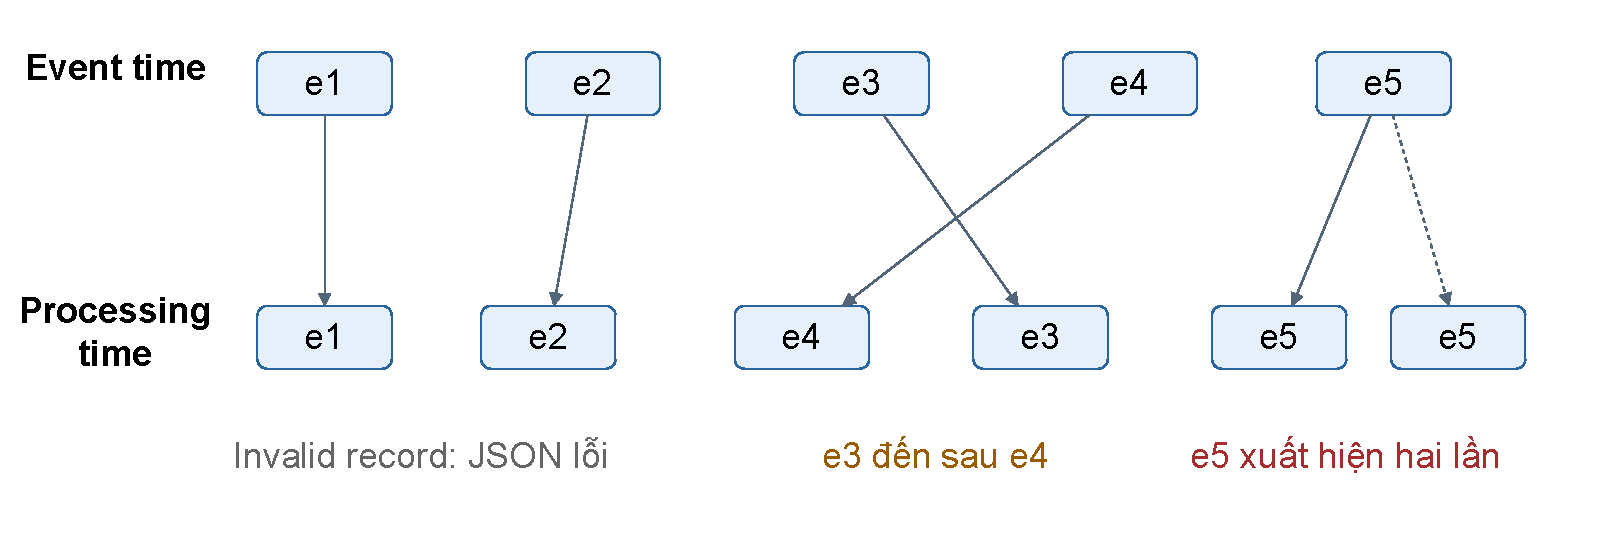
\includegraphics[width=\linewidth]{so-do/theory-01-event-time.pdf}
\caption{Event time và processing time. Mỗi mũi tên nối lúc sự kiện xảy ra với lúc hệ thống xử lý. Sự kiện có thể đến
\textcolor{wpamber}{muộn và lộn thứ tự} (e3), \textcolor{wpred}{đến hai lần} khi nguồn gửi lại (e5), hoặc đến ở dạng
hỏng không đọc được.}\label{fig:eventtime}
\end{figure}

Nếu đếm theo processing time, kết quả phụ thuộc vào việc mạng nhanh hay chậm, và chạy lại cùng dữ liệu sẽ ra số khác.
WikiPulse dùng \textbf{event time} để xếp event vào window theo thời điểm nguồn. Kết quả vẫn phụ thuộc dữ liệu đầu vào, watermark, trạng thái và thứ tự đến; replay không tự bảo đảm cùng kết quả trong mọi điều kiện. Hệ thống cần xử lý late event, bản trùng và bản ghi hỏng. Các mục sau giải thích cách làm từng việc.

\section{Luồng sự kiện thay đổi của Wikipedia}
Wikimedia công bố mọi thay đổi trên các dự án của mình qua dịch vụ EventStreams~\cite{eventstreams}. Client mở một kết nối
HTTP dài và nhận từng sự kiện dạng JSON ngay khi nó xảy ra (giao thức Server-Sent Events). Bảng~\ref{tab:recentchange} liệt
kê các thông tin của một sự kiện mà hệ thống dùng tới.

\begin{table}[H]
\centering\small
\renewcommand{\arraystretch}{1.18}
\caption{Thông tin chính trong một sự kiện thay đổi và cách hệ thống dùng}\label{tab:recentchange}
\begin{tabularx}{\linewidth}{@{}lXX@{}}
\toprule
\textbf{Thông tin} & \textbf{Ý nghĩa} & \textbf{Dùng để} \\ \midrule
Định danh sự kiện & Duy nhất cho mỗi sự kiện & Loại bản trùng \\
Thời điểm & Lúc thay đổi xảy ra (event time) & Xếp vào cửa sổ thời gian \\
Wiki, trang & Ví dụ \enquote{enwiki}, tên bài viết & Nhóm kết quả theo wiki, theo trang \\
Loại thay đổi & Sửa trang, tạo trang mới, ghi nhật ký & Đếm từng loại \\
Kích thước trước, sau & Số byte của trang & Phát hiện xóa nhiều nội dung \\
Người sửa, cờ ẩn danh, cờ bot & Tài khoản hoặc địa chỉ IP và các cờ & Silver băm user với salt; giữ các cờ. Bronze raw giữ payload nguồn \\
\bottomrule
\end{tabularx}
\end{table}

Kết nối dài có thể đứt. Khi nối lại, client có thể nhận lại một phần sự kiện đã nhận, nên phía sau phải chịu được bản
trùng. Ngoài sự kiện thật, Wikimedia còn phát định kỳ \textbf{sự kiện canary} để tự kiểm tra hệ thống của họ; các sự
kiện này phải bị loại khỏi số liệu.
Collector dùng ACK liên tiếp của Kafka để chọn SSE ID khi reconnect trong cùng tiến trình. Cursor chỉ ở bộ nhớ; restart hoặc nguồn không còn giữ vị trí có thể dẫn tới thiếu, trong khi retry có thể tạo bản trùng. Không cam kết exactly-once.

\section{Apache Kafka: bộ đệm sự kiện bền vững}
Kafka~\cite{kreps2011} lưu sự kiện thành một \textbf{nhật ký chỉ ghi thêm} (append-only log). Các khái niệm chính
(Hình~\ref{fig:kafka}):
\begin{itemize}
  \item \textbf{Topic}: một kênh sự kiện, ví dụ kênh chứa các thay đổi thô của Wikipedia.
  \item \textbf{Partition}: topic được chia thành nhiều nhật ký song song để chia tải. Mỗi sự kiện trong một partition có
        số thứ tự tăng dần gọi là \textbf{offset}.
  \item \textbf{Key}: producer gắn key cho mỗi sự kiện; với partitioner và số partition không đổi, cùng key được định tuyến vào cùng partition. Thứ tự được hiểu trong partition, không phải bảo đảm thứ tự toàn hệ thống. WikiPulse dùng key theo wiki và trang.
  \item \textbf{Consumer} tự nhớ mình đã đọc đến offset nào, nên có thể dừng rồi đọc tiếp, hoặc đọc lại từ đầu.
\end{itemize}

\begin{figure}[H]
\centering
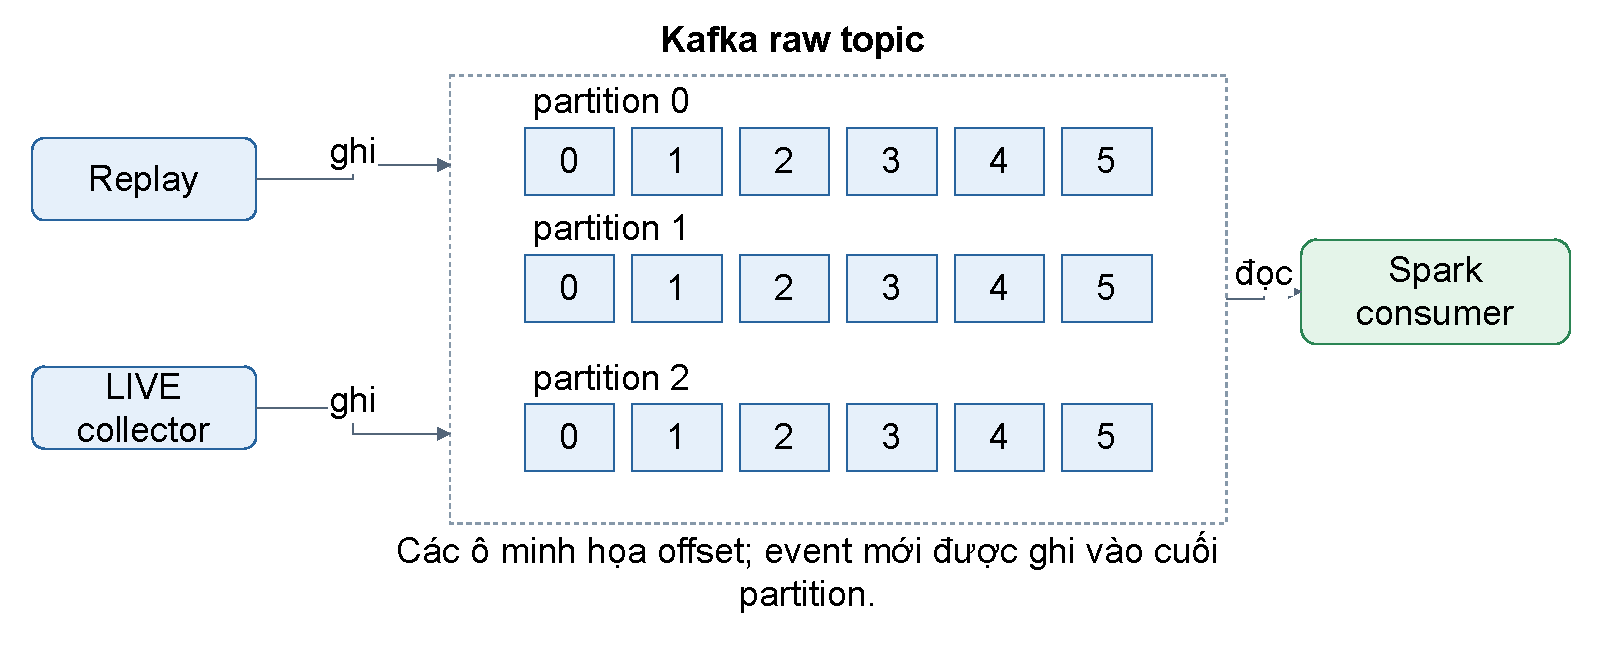
\includegraphics[width=\linewidth]{so-do/theory-02-kafka.pdf}
\caption{Topic Kafka gồm ba partition. Mỗi ô là một sự kiện, số trong ô là offset. Producer ghi vào cuối nhật ký;
consumer (Spark) đọc theo offset và lưu trạng thái theo checkpoint. Collector LIVE đã được triển khai; khả năng tích hợp đầy đủ vẫn cần nghiệm thu.}\label{fig:kafka}
\end{figure}

Trong WikiPulse, Kafka đứng giữa nguồn sự kiện và Spark. Khi Spark dừng, Kafka có thể giữ dữ liệu trong phạm vi retention và trạng thái broker; Spark có thể phục hồi từ checkpoint hợp lệ nếu dữ liệu còn tồn tại. REPLAY ghi fixture vào cùng topic để kiểm thử phần xử lý phía sau; kết quả còn phụ thuộc cấu hình và trạng thái của lần chạy.

\section{Spark Structured Streaming}
\subsection{Mô hình micro-batch}
Spark Structured Streaming~\cite{armbrust2018} cho phép viết truy vấn trên luồng giống như truy vấn trên một bảng bình
thường. Stream được coi là một \textbf{bảng không giới hạn}, mỗi event mới là một dòng thêm vào. Spark dùng trigger
có khoảng mặc định 10 giây trong WikiPulse để lấy dữ liệu mới thành một \textbf{micro-batch}, tính từ state lần trước rồi
ghi kết quả ra đích (Hình~\ref{fig:microbatch}). Nếu batch xử lý lâu, nhịp thực tế có thể chậm hơn cấu hình.

\begin{figure}[H]
\centering
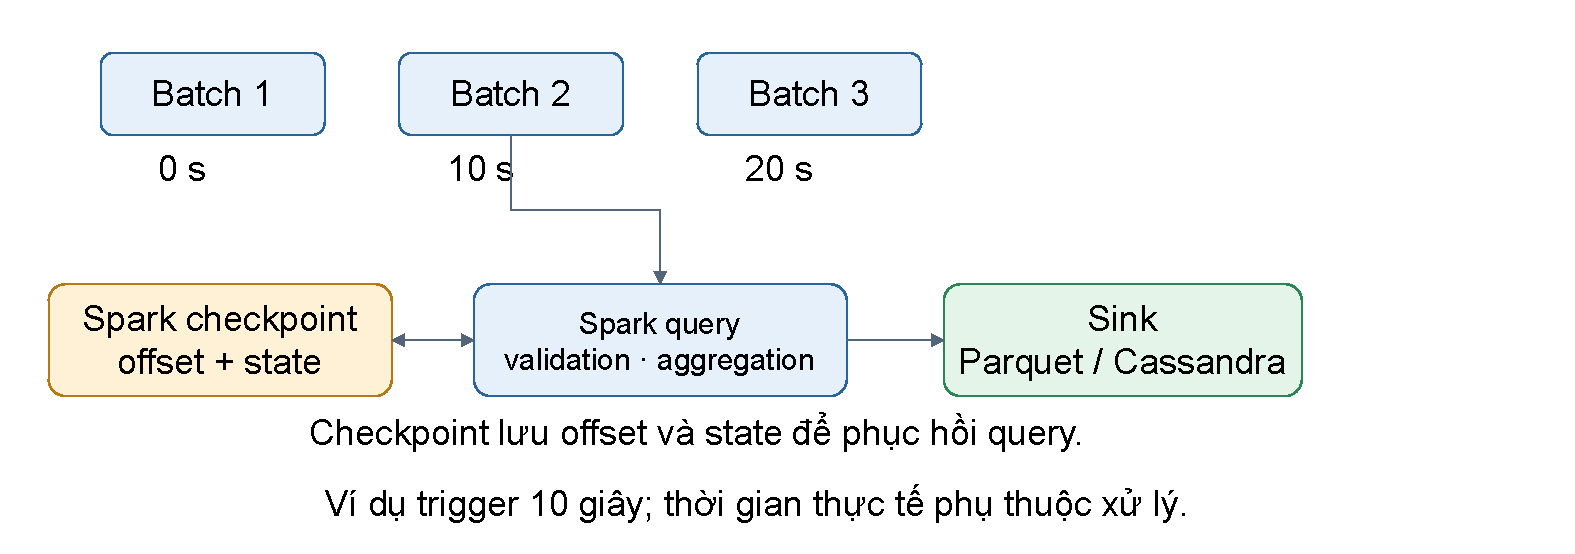
\includegraphics[width=\linewidth]{so-do/theory-03-microbatch.pdf}
\caption{Mô hình micro-batch với trigger mặc định 10 giây; thời điểm thực tế phụ thuộc thời gian xử lý. Query kết hợp batch với state trong checkpoint.}\label{fig:microbatch}
\end{figure}

\textbf{Checkpoint} lưu hai thứ: đã đọc Kafka tới offset nào, và trạng thái đang tính dở (ví dụ số đếm của các cửa sổ chưa
chốt). Spark có thể phục hồi từ checkpoint hợp lệ nếu nguồn còn dữ liệu và state/schema tương thích. Checkpoint gắn chặt với cấu trúc
truy vấn: đổi cách tính có trạng thái thì phải dùng checkpoint mới.

\subsection{Window và watermark}
Để đếm \enquote{mỗi phút có bao nhiêu chỉnh sửa}, sự kiện được xếp vào các \textbf{cửa sổ} 1 phút theo event time. Câu hỏi
khó là: \emph{khi nào thì một cửa sổ được coi là đủ?} Sự kiện của phút 00:00 có thể vẫn đang trên đường tới. Spark trả
lời bằng \textbf{watermark}~\cite{akidau2015}:
\[
  \text{watermark} = \text{event time lớn nhất đã thấy} - \text{độ trễ cho phép (10 phút)}.
\]
Khi watermark tiến qua cuối window, query có thể xuất kết quả finalized theo output mode. Sự kiện đến quá muộn có thể bị loại khỏi phép tính có state, trong khi Bronze raw vẫn giữ bản ghi Kafka. Watermark dựa trên event time quan sát được và tiến độ query, không phải timer theo đồng hồ; khi stream im lặng không thể giả định Gold lập tức được chốt.
Hình~\ref{fig:watermark} minh họa bằng chính dữ liệu mẫu của dự án.

\begin{figure}[H]
\centering
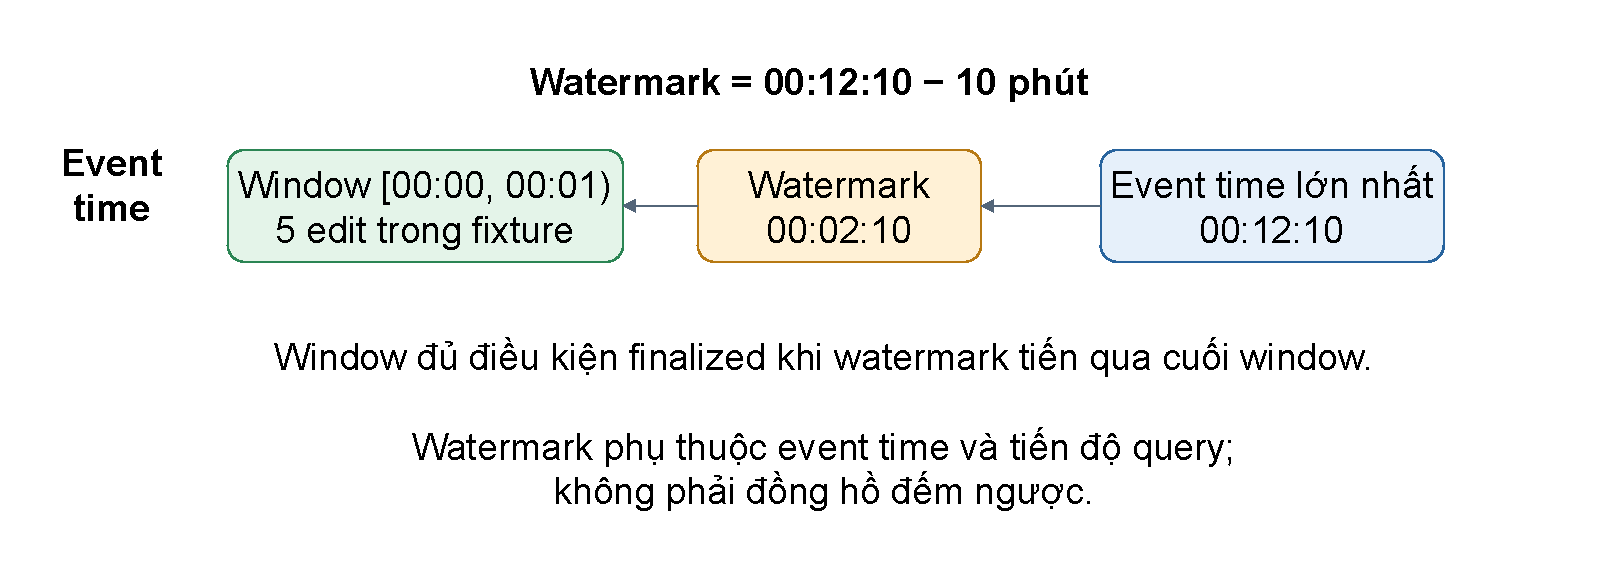
\includegraphics[width=\linewidth]{so-do/theory-04-watermark.pdf}
\caption{Watermark trên dữ liệu mẫu. Sự kiện lúc 00:12:10 đẩy watermark tới 00:02:10, nên cửa sổ 00:00 (5 chỉnh sửa
enwiki) được chốt. Các window có cuối sau watermark này chưa đủ điều kiện finalized chỉ dựa trên mốc đó.}\label{fig:watermark}
\end{figure}

Độ trễ cho phép là một sự đánh đổi: dài thì đếm được nhiều sự kiện muộn hơn nhưng phải giữ nhiều trạng thái và chờ lâu
mới có số chốt; ngắn thì ngược lại. Dự án chọn 10 phút.

\subsection{Số tạm tính và số đã chốt}
Người xem dashboard muốn thấy số ngay, không muốn chờ 10 phút. Spark có hai \textbf{chế độ xuất} kết quả, và WikiPulse
dùng cả hai cho cùng một phép đếm (Bảng~\ref{tab:chedo}).

\begin{table}[H]
\centering\small
\caption{Hai chế độ xuất kết quả}\label{tab:chedo}
\begin{tabularx}{\linewidth}{@{}lXXX@{}}
\toprule
\textbf{Chế độ} & \textbf{Khi nào ghi} & \textbf{Tính chất} & \textbf{Đích trong WikiPulse} \\ \midrule
Update & Mỗi batch, mọi cửa sổ vừa thay đổi & Nhanh; số còn có thể tăng (tạm tính) & Activity: Cassandra; trends: Parquet hoặc Cassandra theo cấu hình \\
Append & Khi window đủ điều kiện theo watermark & Kết quả finalized; thời điểm xuất phụ thuộc tiến độ event time & Tầng Gold, cho phân tích \\
\bottomrule
\end{tabularx}
\end{table}

Spark có một giới hạn quan trọng: một truy vấn ở chế độ Update không được chứa hai bước cần nhớ trạng thái liên tiếp, ví
dụ \enquote{loại trùng rồi đếm}~\cite{sparkguide}. Vì vậy WikiPulse tách thành nhiều truy vấn: một truy vấn loại trùng và
ghi ra đĩa, các truy vấn khác đọc lại kết quả đó để đếm (Mục~\ref{sec:spark}).

\subsection{Loại bản trùng}
Mỗi sự kiện có một định danh duy nhất. Spark nhớ các định danh đã thấy và bỏ sự kiện nào trùng. Không thể nhớ mãi, nên
Spark dùng event ID và state có watermark để deduplication trong phạm vi cấu hình. Bản trùng đến muộn có thể bị bỏ vì quá muộn hoặc không còn được nhận diện là trùng; không khẳng định chính xác kết quả mọi trường hợp hay exactly-once.

\section{Kiến trúc dữ liệu ba tầng}
Thay vì chỉ lưu kết quả cuối, dữ liệu được lưu theo ba tầng~\cite{medallion}, mỗi tầng sạch hơn tầng trước
(Hình~\ref{fig:medallion}). Lưu tầng thô giúp kiểm tra lại khi nghi có lỗi và tính lại khi đổi công thức mà không cần nguồn
gửi lại dữ liệu.

\begin{figure}[H]
\centering
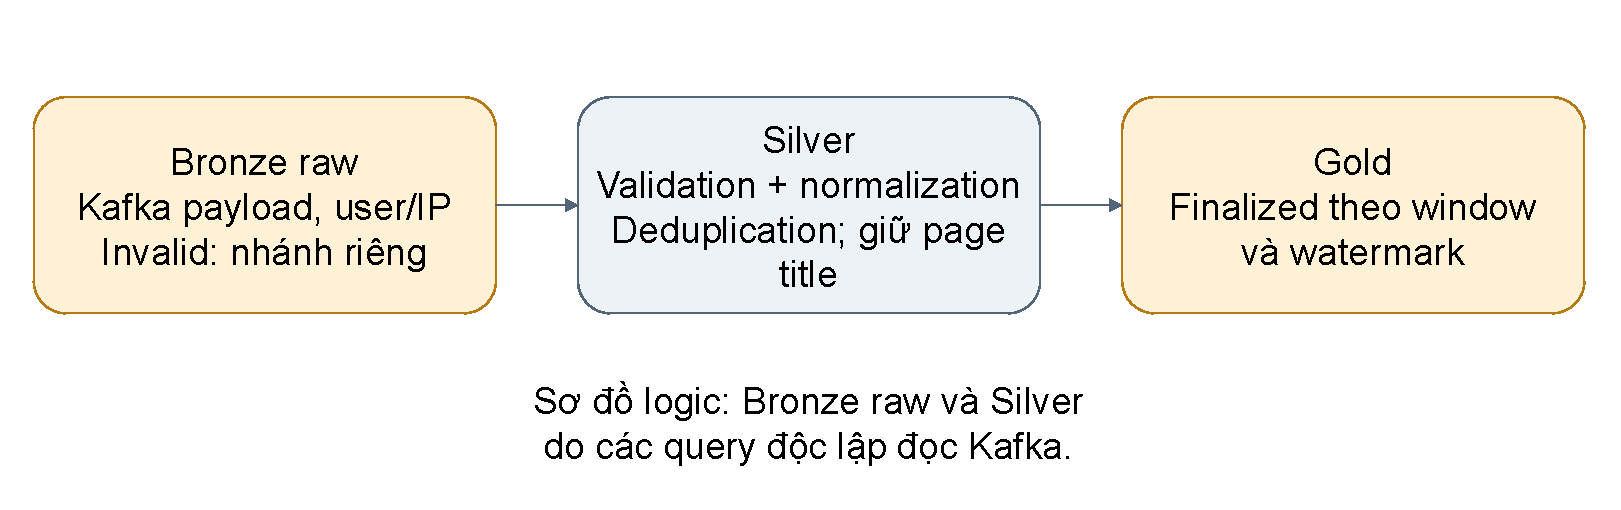
\includegraphics[width=\linewidth]{so-do/theory-05-medallion.pdf}
\caption{Ba tầng dữ liệu. Đi từ trái sang phải, dữ liệu sạch dần và ít thông tin nhạy cảm hơn.}\label{fig:medallion}
\end{figure}

Ba tầng được lưu dạng \textbf{Parquet}, định dạng theo cột, nén tốt, đọc nhanh khi chỉ cần vài cột. File được chia thư
mục theo ngày và giờ, nên truy vấn một khoảng thời gian chỉ phải đọc đúng các thư mục đó.

\section{Apache Cassandra: phục vụ kết quả}
Dashboard cần đọc số liệu nhanh, liên tục. Parquet hợp cho phân tích theo lô nhưng không hợp để trả lời hàng nghìn câu
hỏi nhỏ mỗi phút. Kết quả tạm tính vì vậy được ghi vào Cassandra~\cite{lakshman2010}.

Khác CSDL quan hệ, trong Cassandra \textbf{bảng được thiết kế theo câu truy vấn}, không theo thực thể~\cite{cassandracql}.
Khóa chính có hai phần (Hình~\ref{fig:cassandra}):
\begin{itemize}
  \item \textbf{Partition key} quyết định dữ liệu nằm cùng nhau ở đâu. WikiPulse dùng wiki: mọi cửa sổ của enwiki nằm
        chung một partition.
  \item \textbf{Clustering key} quyết định thứ tự trong partition. WikiPulse dùng thời điểm bắt đầu cửa sổ, sắp giảm dần,
        nên các phút mới nhất luôn nằm đầu.
\end{itemize}

\begin{figure}[H]
\centering
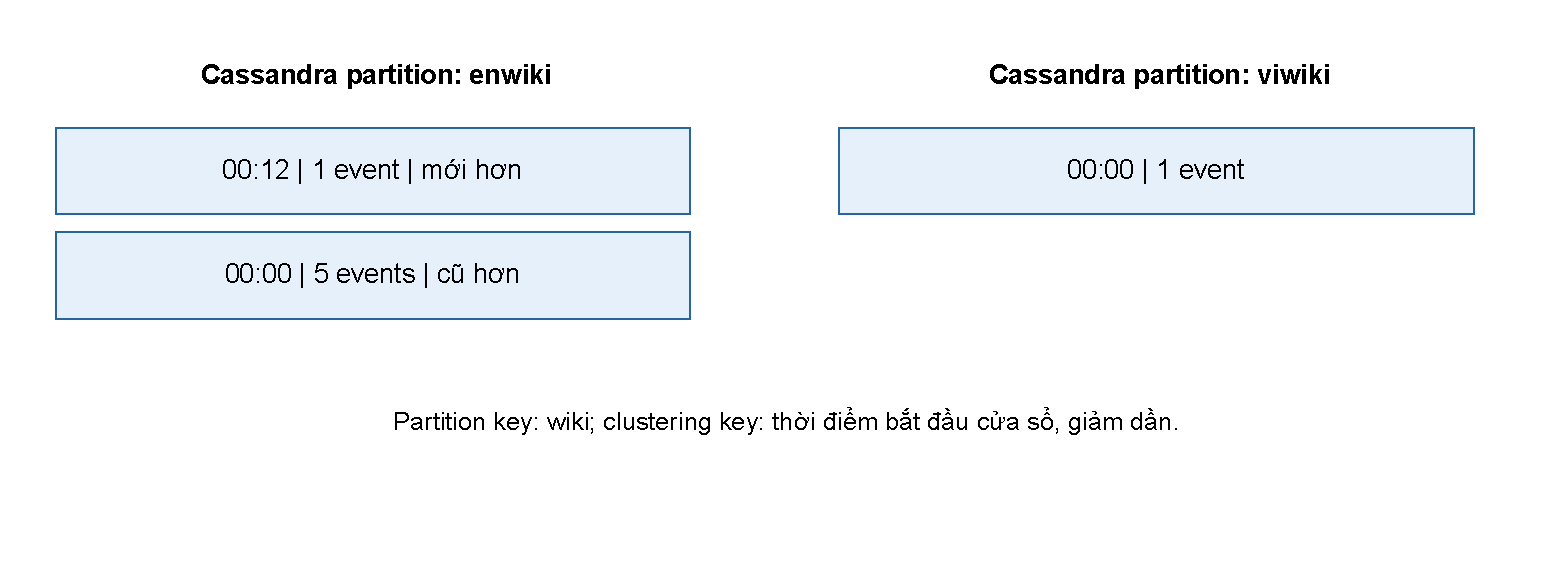
\includegraphics[width=\linewidth]{so-do/theory-06-cassandra.pdf}
\caption{Dữ liệu hoạt động trong Cassandra. Mỗi wiki là một partition; trong partition, các cửa sổ xếp mới trước.}\label{fig:cassandra}
\end{figure}

Hai tính chất của Cassandra quyết định cách ghi:
\begin{itemize}
  \item Ghi một dòng có khóa đã tồn tại thì \textbf{ghi đè} (upsert), không sinh dòng mới. WikiPulse ghi \emph{tổng số}
        của cửa sổ chứ không ghi \enquote{cộng thêm 1}, nên khi Spark ghi lại một batch sau sự cố, kết quả vẫn đúng, không
        bị đếm đôi.
  \item Truy vấn không chỉ rõ partition buộc Cassandra quét mọi node. Dự án cấm kiểu truy vấn này (\enquote{allow
        filtering}); mỗi câu hỏi của API phải có bảng thiết kế riêng cho nó.
\end{itemize}

\section{FastAPI và Streamlit}
\textbf{FastAPI} là framework Python để viết API web; kiểu dữ liệu khai báo một lần được dùng để kiểm tra đầu vào, định
dạng đầu ra và sinh tài liệu API tự động (OpenAPI). \textbf{Streamlit} dựng giao diện dashboard bằng Python thuần, hợp với
nhóm không có người chuyên frontend.

\section{Công nghệ sử dụng}
\begin{table}[H]
\centering\small
\caption{Công nghệ sử dụng và vai trò}\label{tab:congnghe}
\begin{tabularx}{\linewidth}{@{}llX@{}}
\toprule
\textbf{Thành phần} & \textbf{Lựa chọn} & \textbf{Vai trò} \\ \midrule
Hàng đợi & Apache Kafka 3.9 & Giữ sự kiện, tách nguồn khỏi xử lý, cho phép đọc lại \\
Xử lý luồng & Spark 3.5 (PySpark) & Kiểm tra, chuẩn hóa, loại trùng, đếm theo cửa sổ \\
Lưu trữ phân tích & Parquet (local hoặc HDFS) & Ba tầng Bronze, Silver, Gold \\
Lưu trữ phục vụ & Apache Cassandra 4.1 & Số tạm tính cho API \\
API & FastAPI & Cung cấp số liệu cho dashboard \\
Giao diện & Streamlit & Dashboard bốn trang \\
Chạy & Docker Compose & Dựng toàn bộ hệ thống bằng một lệnh, chạy trên ARM64 và x86\_64 \\
Ngôn ngữ, kiểm thử & Python 3.11, pytest & Toàn bộ mã nguồn và kiểm thử \\
\bottomrule
\end{tabularx}
\end{table}
Profile full bổ sung HDFS cho data và Spark checkpoint; cấu hình mặc định vẫn dùng local storage.

% ============================================================================
% CHƯƠNG 3: LIÊN QUAN
% ============================================================================

\chapter{Các hướng tiếp cận liên quan}\label{chap:lienquan}
\section{Theo dõi thay đổi Wikipedia}
Dịch vụ Wikimedia EventStreams công bố luồng thay đổi để các ứng dụng khác tiếp nhận~\cite{eventstreams}. Dữ liệu nguồn cho biết sự kiện đã xảy ra; để quan sát xu hướng theo thời gian, ứng dụng tiếp nhận cần tự lựa chọn cách lọc, tổng hợp và trình bày.
\section{Đánh giá và ưu tiên chỉnh sửa}
Một hướng hỗ trợ người tuần tra là dùng dấu hiệu của chỉnh sửa để sắp xếp thứ tự cần xem. WikiPulse dùng các quy tắc mô tả được, dựa trên mức xóa nội dung, dấu hiệu hoàn tác và tình trạng ẩn danh. Quy tắc đơn giản giúp giải thích kết quả nhưng không thay thế việc xem xét ngữ cảnh của con người.
\section{Phân tích dữ liệu luồng}
Kafka cung cấp lớp lưu và truyền sự kiện~\cite{kreps2011}, còn Spark Structured Streaming hỗ trợ xử lý theo cửa sổ và trạng thái~\cite{armbrust2018}. WikiPulse kết hợp các thành phần này với lưu trữ phân tích và lưu trữ phục vụ truy vấn để đưa kết quả lên giao diện. Xu hướng trong báo cáo phản ánh hoạt động chỉnh sửa, không phải số lượt xem trang.

\chapter{Phân tích, thiết kế và cài đặt}\label{chap:thietke}

\section{Phân tích yêu cầu}
\subsection{Tác nhân}
\begin{itemize}
  \item \textbf{Người xem:} người tuần tra hoặc người quan tâm đến Wikipedia, mở dashboard để xem hoạt động, trang xu
        hướng và các chỉnh sửa nên xem trước. Không cần đăng nhập (ngoài phạm vi MVP).
  \item \textbf{Người vận hành:} thành viên nhóm khởi động, dừng hệ thống, phát lại dữ liệu mẫu, chuyển sang nguồn thật
        và kiểm tra trạng thái. Người vận hành làm được mọi việc của người xem.
  \item \textbf{Wikimedia EventStreams (hệ thống ngoài):} phát luồng sự kiện thay đổi ở chế độ LIVE.
\end{itemize}

\subsection{Biểu đồ use case}
\begin{figure}[H]
\centering
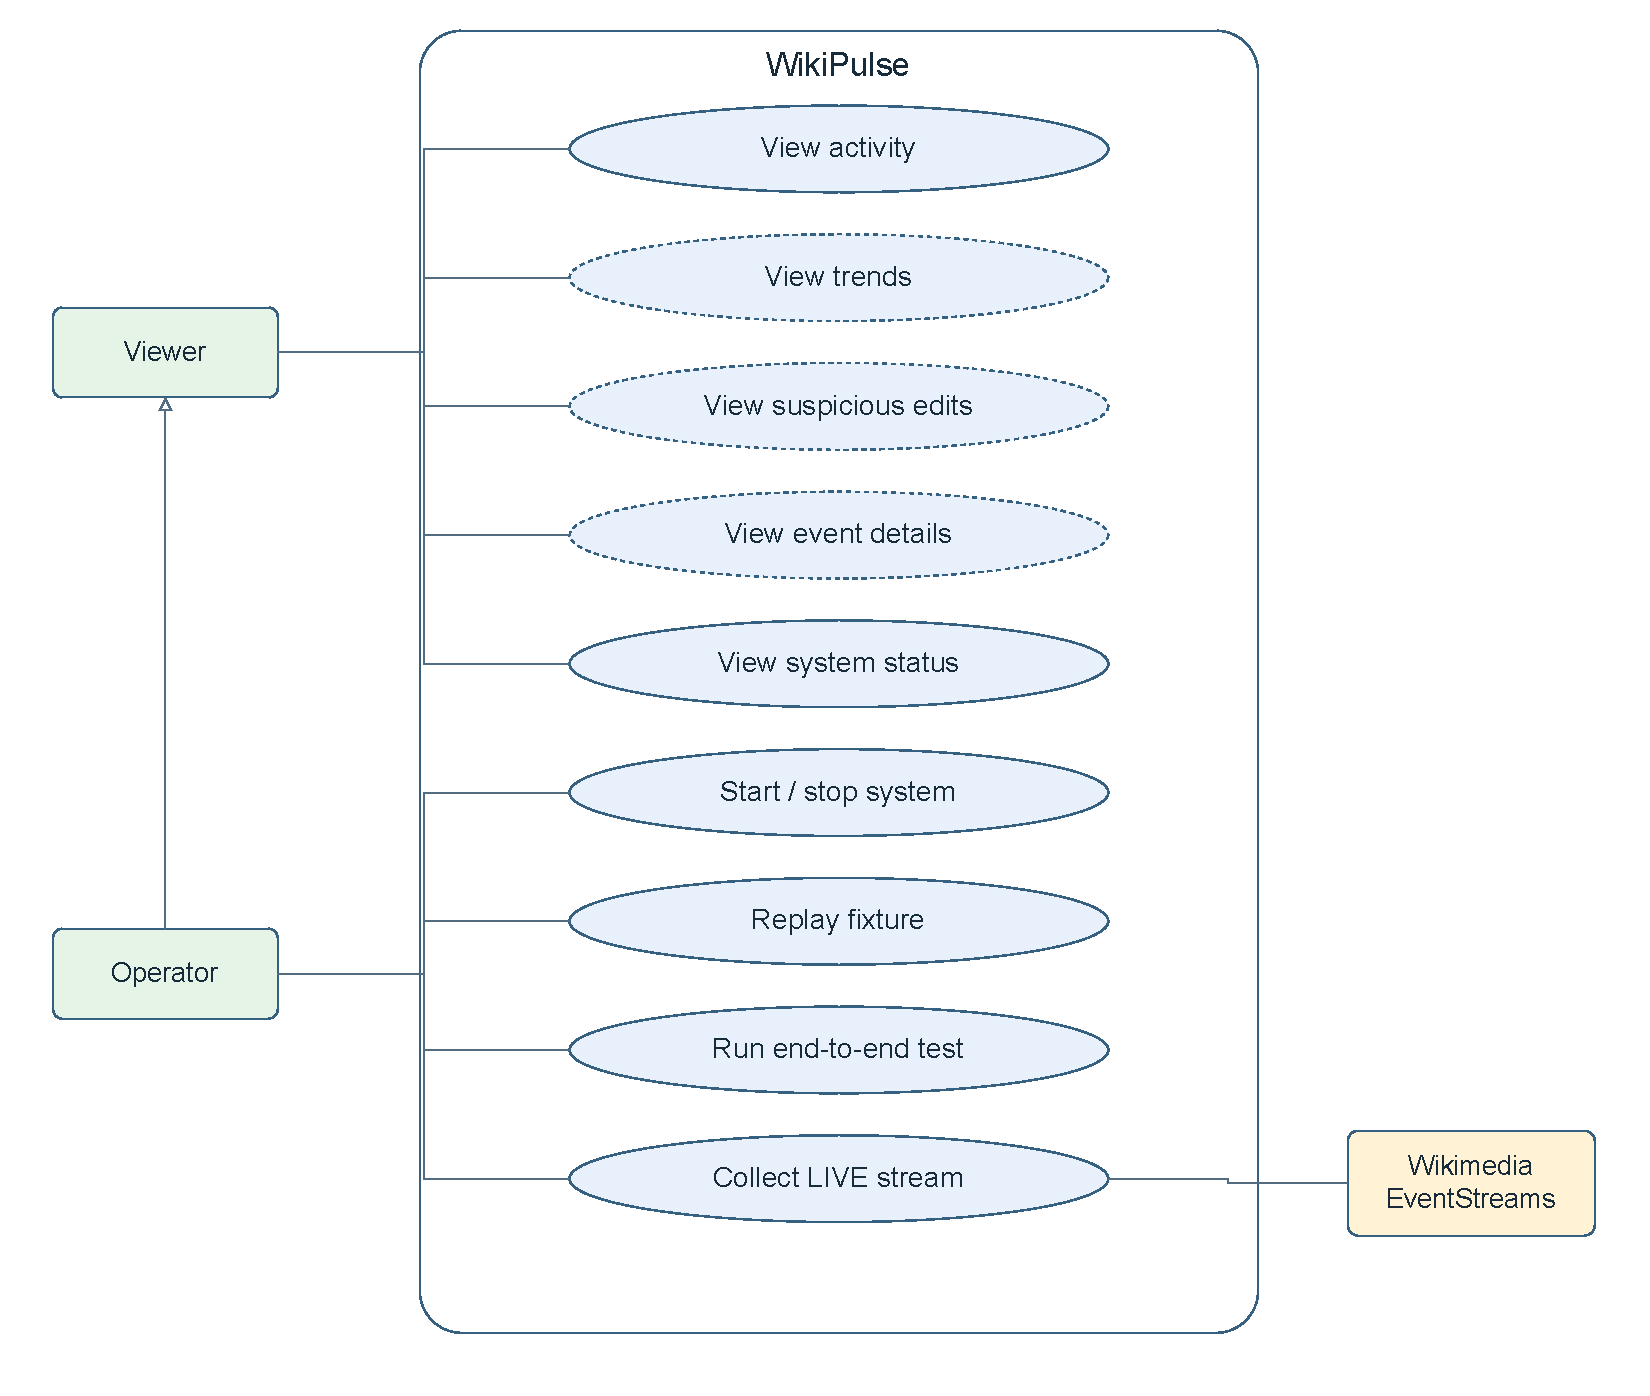
\includegraphics[width=\linewidth,height=0.68\textheight,keepaspectratio]{so-do/design-usecase.pdf}
\caption{Biểu đồ use case tổng quát. Đường nối là quan hệ giữa tác nhân và use case; mũi tên tam giác rỗng là quan hệ
khái quát hóa (người vận hành làm được mọi việc của người xem). Viền đứt nét đánh dấu phần giao diện chưa hoàn thiện;
collector LIVE đã được thử riêng, không suy ra LIVE end-to-end đã nghiệm thu.}\label{fig:usecase}
\end{figure}
\dukiensua{Mạnh đối chiếu trạng thái dashboard và use case trước khi chốt.}

\subsection{Đặc tả các use case chính}
\begin{table}[H]
\centering\small
\caption{Đặc tả use case \enquote{Xem hoạt động theo wiki}}\label{tab:uc-hoatdong}
\begin{tabularx}{\linewidth}{@{}>{\bfseries}p{3.2cm}X@{}}
\toprule
Tác nhân & Người xem \\
Tiền điều kiện & Hệ thống đang chạy \\
Luồng chính & 1. Người xem mở trang Overview, chọn wiki (mặc định enwiki).\newline
2. Dashboard gọi API lấy các cửa sổ 1 phút mới nhất của wiki đó.\newline
3. API đọc đúng partition của wiki trong Cassandra và trả kết quả, gắn nhãn \enquote{tạm tính}.\newline
4. Dashboard hiện năm chỉ số (sự kiện, chỉnh sửa, trang mới, sửa ẩn danh, sửa bởi bot) và biểu đồ theo thời gian;
tự làm mới sau 15 giây.\newline
5. Người xem có thể chọn một cửa sổ cụ thể để xem riêng. \\
Luồng thay thế & 3a. Chưa có dữ liệu: hiện thông báo trống, không hiện số giả.\newline
3b. Cassandra không phản hồi: API trả lỗi \enquote{phụ thuộc chưa sẵn sàng}; dashboard báo dịch vụ chưa sẵn sàng.\newline
1a. Wiki không nằm trong danh sách cho phép: API từ chối yêu cầu. \\
Hậu điều kiện & Không thay đổi dữ liệu \\
\bottomrule
\end{tabularx}
\end{table}

\begin{table}[H]
\centering\small
\caption{Đặc tả use case \enquote{Phát lại dữ liệu mẫu}}\label{tab:uc-replay}
\begin{tabularx}{\linewidth}{@{}>{\bfseries}p{3.2cm}X@{}}
\toprule
Tác nhân & Người vận hành \\
Tiền điều kiện & Kafka đã sẵn sàng và đã có topic \\
Luồng chính & 1. Người vận hành chạy lệnh phát lại.\newline
2. Hệ thống đọc từng dòng của file dữ liệu mẫu, giữ nguyên định danh và thời điểm của sự kiện, thêm thời điểm nhận.\newline
3. Hệ thống gửi từng sự kiện vào Kafka với khóa wiki và trang, chờ Kafka xác nhận.\newline
4. Spark xử lý sự kiện; nếu cấu hình và các dịch vụ phục vụ sẵn sàng, dashboard có thể hiển thị kết quả. \\
Luồng thay thế & 2a. Dòng không phải JSON hợp lệ: vẫn gửi nguyên văn để kiểm tra đường xử lý bản ghi hỏng.\newline
1a. Người vận hành chọn tốc độ phát nhanh hơn: chỉ đổi nhịp gửi, không đổi thời điểm sự kiện. \\
Hậu điều kiện & Kafka có thêm các sự kiện mẫu; Spark deduplicate theo event ID trong phạm vi watermark \\
\bottomrule
\end{tabularx}
\end{table}

\begin{table}[H]
\centering\small
\caption{Đặc tả use case \enquote{Xem trang xu hướng}}\label{tab:uc-xuhuong}
\begin{tabularx}{\linewidth}{@{}>{\bfseries}p{3.2cm}X@{}}
\toprule
Tác nhân & Người xem \\
Tiền điều kiện & Hệ thống đang chạy, Spark ghi kết quả xu hướng vào Cassandra \\
Luồng chính & 1. Người xem mở trang Trending, chọn wiki.\newline
2. Dashboard gọi API lấy top-N trang của cửa sổ 5 phút mới nhất.\newline
3. API tra bảng chỉ mục để biết cửa sổ mới nhất của wiki, đọc toàn bộ các trang trong cửa sổ đó, sắp theo điểm xu
hướng giảm dần (hòa thì theo số chỉnh sửa, rồi theo mã trang) và trả N dòng đầu kèm mốc đầu, cuối của cửa sổ.\newline
4. Dashboard hiện bảng trang xu hướng, gắn nhãn \enquote{tạm tính}. \\
Luồng thay thế & 2a. Người xem chọn một cửa sổ cụ thể: API đọc đúng cửa sổ đó.\newline
3a. Chưa có cửa sổ nào: trả danh sách rỗng, mốc cửa sổ để trống.\newline
3b. Cửa sổ có hơn 5.000 trang: API báo vượt dung lượng thay vì trả bảng xếp hạng bị cắt.\newline
3c. Cassandra không phản hồi: API báo \enquote{phụ thuộc chưa sẵn sàng}. \\
Hậu điều kiện & Không thay đổi dữ liệu \\
\bottomrule
\end{tabularx}
\end{table}

\begin{table}[H]
\centering\small
\caption{Đặc tả use case \enquote{Xem chỉnh sửa cần ưu tiên}}\label{tab:uc-uutien}
\begin{tabularx}{\linewidth}{@{}>{\bfseries}p{3.2cm}X@{}}
\toprule
Tác nhân & Người xem \\
Tiền điều kiện & Hệ thống đang chạy, Spark ghi các chỉnh sửa có điểm ưu tiên lớn hơn 0 vào Cassandra \\
Luồng chính & 1. Người xem mở trang Suspicious Edits, chọn wiki, số phút gần nhất (1--15) và điểm tối thiểu.\newline
2. Dashboard gọi API.\newline
3. API lấy danh sách các phút có chỉnh sửa đáng chú ý trong khoảng đã chọn từ bảng chỉ mục, đọc từng phút, lọc theo
điểm tối thiểu, sắp theo điểm rồi theo thời điểm giảm dần.\newline
4. Dashboard hiện danh sách kèm lý do (xóa nhiều nội dung, hoàn tác, sửa ẩn danh) và câu nhắc \enquote{điểm dùng để
ưu tiên xem xét, không kết luận phá hoại}. \\
Luồng thay thế & 3a. Không có chỉnh sửa nào: trả danh sách rỗng.\newline
3b. Tổng số dòng các phút cần đọc vượt 5.000: API báo vượt dung lượng.\newline
1a. Số phút hoặc điểm tối thiểu ngoài giới hạn: API từ chối, chỉ rõ tham số sai. \\
Hậu điều kiện & Không thay đổi dữ liệu; phản hồi không có trường user, IP, comment hoặc user hash; page title có thể chứa thông tin nhận dạng \\
\bottomrule
\end{tabularx}
\end{table}

\begin{table}[H]
\centering\small
\caption{Đặc tả use case \enquote{Xem chi tiết một sự kiện}}\label{tab:uc-chitiet}
\begin{tabularx}{\linewidth}{@{}>{\bfseries}p{3.2cm}X@{}}
\toprule
Tác nhân & Người xem \\
Tiền điều kiện & Người xem có định danh sự kiện, thường lấy từ danh sách chỉnh sửa cần ưu tiên \\
Luồng chính & 1. Người xem chọn một sự kiện.\newline
2. API đọc đúng một dòng theo định danh sự kiện.\newline
3. API trả thông tin trang, phiên bản cũ và mới, độ dài, chênh lệch byte, các cờ ẩn danh, bot, sửa nhỏ, điểm và lý
do ưu tiên. \\
Luồng thay thế & 2a. Không tìm thấy (sai định danh, hoặc sự kiện cũ hơn 7 ngày đã hết hạn lưu): API trả lỗi
\enquote{không tìm thấy sự kiện}.\newline
3a. Sự kiện không dính dấu hiệu nào: điểm 0, danh sách lý do rỗng. \\
Hậu điều kiện & Không thay đổi dữ liệu \\
\bottomrule
\end{tabularx}
\end{table}
\dukiensua{Bước hiển thị trên dashboard của ba use case trên làm ở W2-MANH-01; phần API đã chạy.}
\subsubsection{Đặc tả use case \enquote{Thu thập luồng thật (LIVE)}}
Collector kết nối Wikimedia EventStreams, nhận sự kiện qua SSE và gửi vào Kafka raw topic. Khi kết nối gián đoạn,
collector thử reconnect và gửi \code{Last-Event-ID} của sự kiện cuối đã được Kafka xác nhận theo thứ tự. Cursor chỉ
được giữ trong bộ nhớ process, vì vậy restart bắt đầu từ stream hiện tại. Việc nghiệm thu LIVE end-to-end của nhóm
vẫn còn chờ; kết quả collector riêng được trình bày trong chương kiểm thử.
\dukiensua{Đối chiếu contract và review cùng Thành, Linh trước khi nghiệm thu.}

\subsection{Yêu cầu chức năng}
\begin{table}[H]
\centering\small
\caption{Yêu cầu chức năng và trạng thái}\label{tab:ycchucnang}
\begin{tabularx}{\linewidth}{@{}lXl@{}}
\toprule
\textbf{Mã} & \textbf{Yêu cầu} & \textbf{Trạng thái} \\ \midrule
F1 & Phát lại dữ liệu mẫu vào Kafka, giữ nguyên định danh và thời điểm sự kiện & Đã làm \\
F2 & Nhận luồng thật từ Wikimedia, tự nối lại khi mất kết nối & Collector đã thử \\
F3 & Kiểm tra, tách riêng bản ghi hỏng, chuẩn hóa, loại trùng & Đã làm \\
F4 & Đếm hoạt động theo wiki, cửa sổ 1 phút; có số tạm tính và số đã chốt & Đã làm \\
F5 & Trang xu hướng: cửa sổ 5 phút trượt mỗi 1 phút, top-N theo wiki & API đã làm \\
F6 & Ưu tiên xem xét chỉnh sửa theo ba dấu hiệu: xóa nhiều nội dung, hoàn tác qua lại, sửa ẩn danh & API đã làm \\
F7 & Tra cứu chi tiết một sự kiện & API đã làm \\
F8 & Dashboard 4 trang: Overview, Trending, Suspicious Edits, System Status & Overview đã làm \\
F9 & Lưu ba tầng trên HDFS & Đã thử REPLAY \\
\bottomrule
\end{tabularx}
\end{table}
\dukiensua{Cập nhật trạng thái theo từng checkpoint.}

\subsection{Yêu cầu phi chức năng}
\begin{itemize}
  \item \textbf{Độ trễ:} số tạm tính hiện trên API trong 30--60 giây ở tải demo (mục tiêu, chưa đo). Số đã chốt chậm hơn
        theo watermark 10 phút.
  \item \textbf{Đúng khi chạy lại:} kiểm tra retry và restart theo từng fixture; không suy ra exactly-once giữa các sink.
  \item \textbf{Riêng tư:} Silver loại trường user/comment gốc và dùng salted hash cho user; page title và metadata
        vẫn có thể chứa thông tin nhận dạng. Pseudonymization không bảo đảm anonymity hoàn toàn.
  \item \textbf{Tái hiện:} lệnh và điều kiện được ghi trong plan; một số lượt cần artifact local hoặc môi trường riêng.
  \item \textbf{Tài nguyên:} chạy được trên máy 16 GB RAM, cấp cho Docker 6--8 GB.
\end{itemize}

\section{Kiến trúc tổng quan}
\begin{figure}[H]
\centering
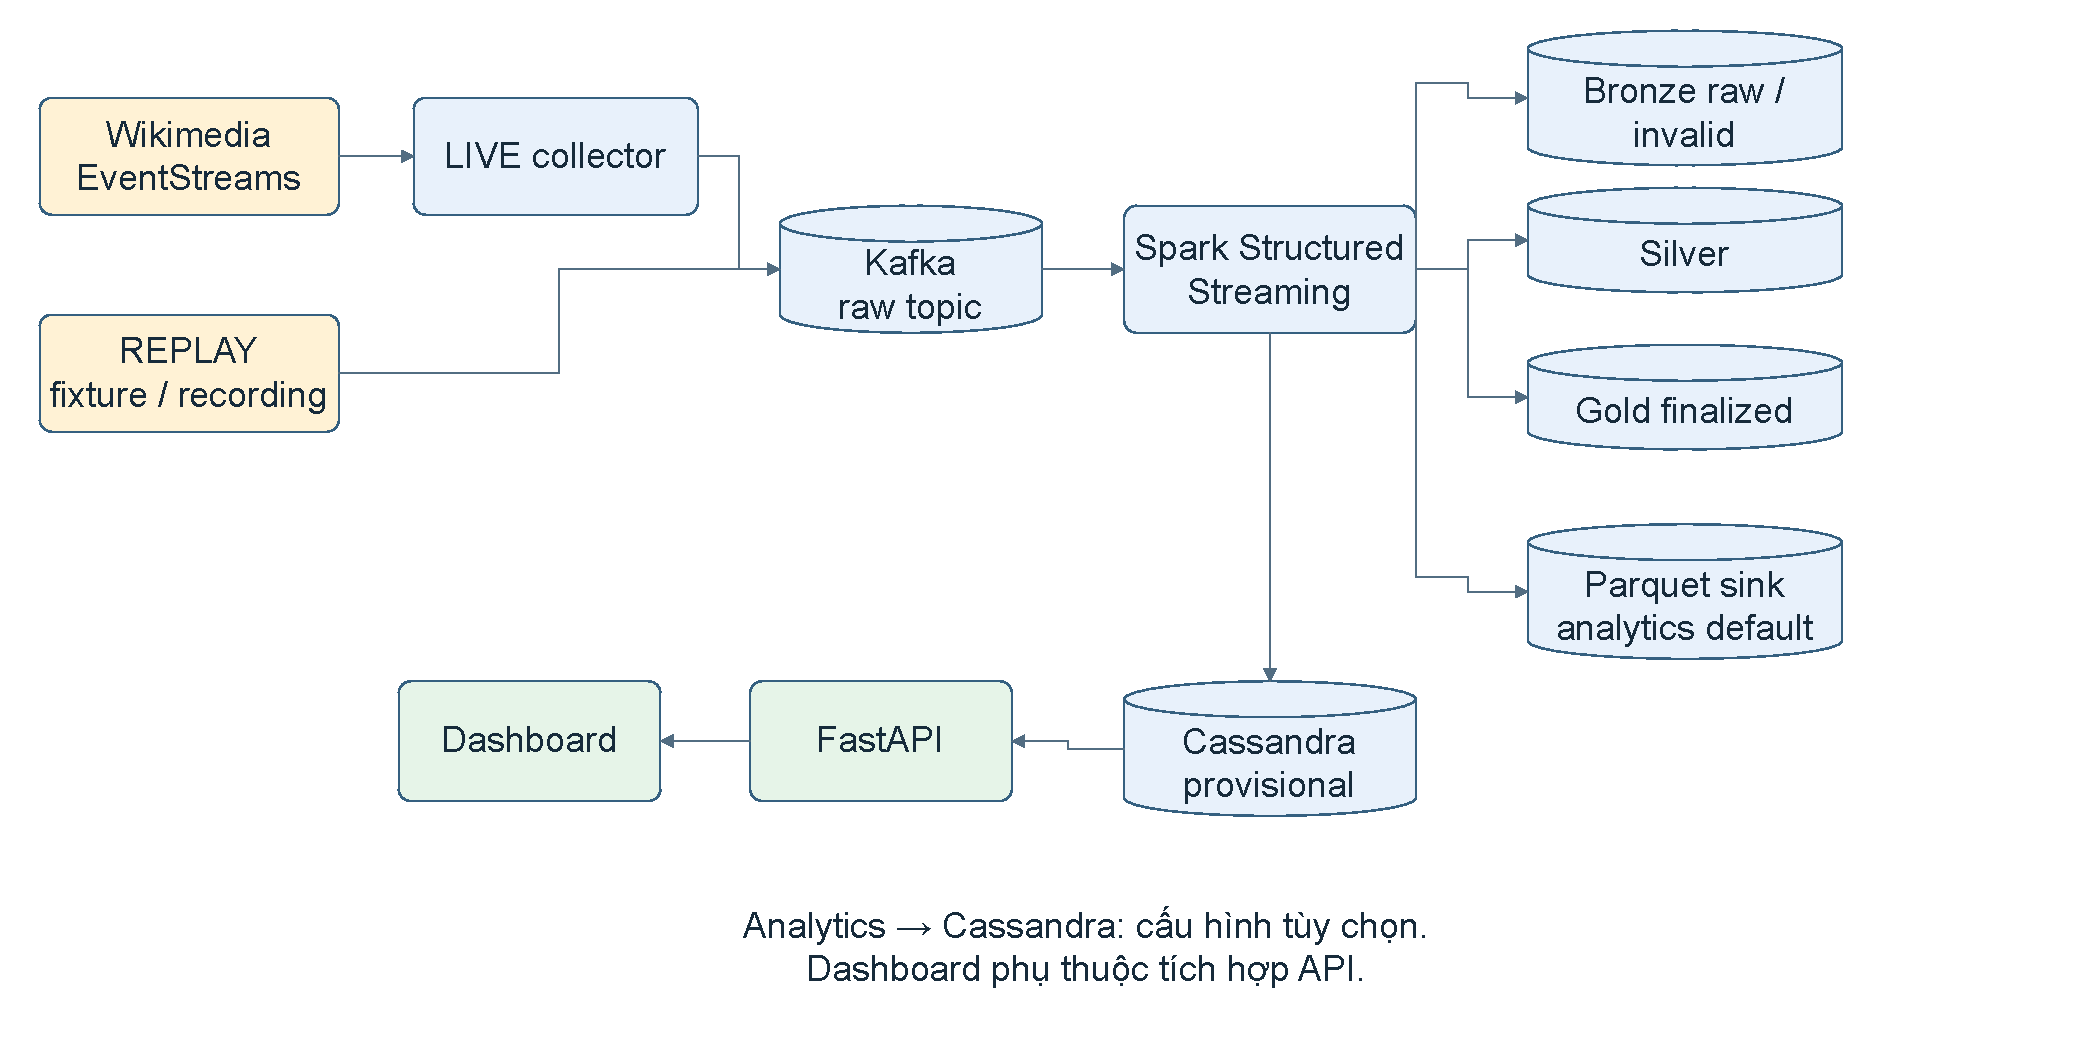
\includegraphics[width=\linewidth,height=0.68\textheight,keepaspectratio]{so-do/design-architecture.pdf}
\caption{Sơ đồ kiến trúc tổng quan. Collector LIVE đã được thử riêng với Kafka; sơ đồ không khẳng định toàn bộ luồng
LIVE tới dashboard đã được nghiệm thu. Màu xanh dương là xử lý, xanh lá là đầu ra, vàng là nguồn bên ngoài.}\label{fig:kientruc}
\end{figure}

Kafka tách phần nhận khỏi phần xử lý; Spark chuẩn hóa và tính các kết quả nghiệp vụ, API và dashboard đọc kết quả.
Dashboard gọi API thay vì đọc Cassandra trực tiếp. Theo cấu hình mặc định, analytics sink là Parquet; Cassandra cho
trends, suspicious edits và event detail phải được chọn trong cấu hình. API đã cài đặt không đồng nghĩa dashboard đã
kết nối đầy đủ hoặc dữ liệu có sẵn trong cấu hình mặc định.

\subsection{Các thành phần và người phụ trách}
\begin{table}[H]
\centering\small
\caption{Các thành phần (vị trí mã nguồn ở Phụ lục~\ref{app:ma})}\label{tab:module}
\begin{tabularx}{\linewidth}{@{}lXl@{}}
\toprule
\textbf{Thành phần} & \textbf{Nhiệm vụ} & \textbf{Phụ trách} \\ \midrule
Lõi dùng chung & Đọc và kiểm tra cấu hình, ghi log dạng JSON, lớp truy cập Cassandra & Trọng, Nhân \\
Thu thập & Phát lại dữ liệu mẫu, thu thập luồng thật & Thành \\
Xử lý & Tiến trình Spark: các truy vấn, phép biến đổi, giám sát truy vấn & Linh \\
Ghi kết quả & Đưa số đếm từ Spark vào Cassandra & Nhân \\
Phục vụ & Lược đồ Cassandra, API & Nhân \\
Giao diện & Dashboard và lớp gọi API & Mạnh \\
Tích hợp & Docker Compose, tạo topic, dữ liệu mẫu, kiểm thử end-to-end & Trọng \\
\bottomrule
\end{tabularx}
\end{table}

\subsection{Triển khai}
\begin{figure}[H]
\centering
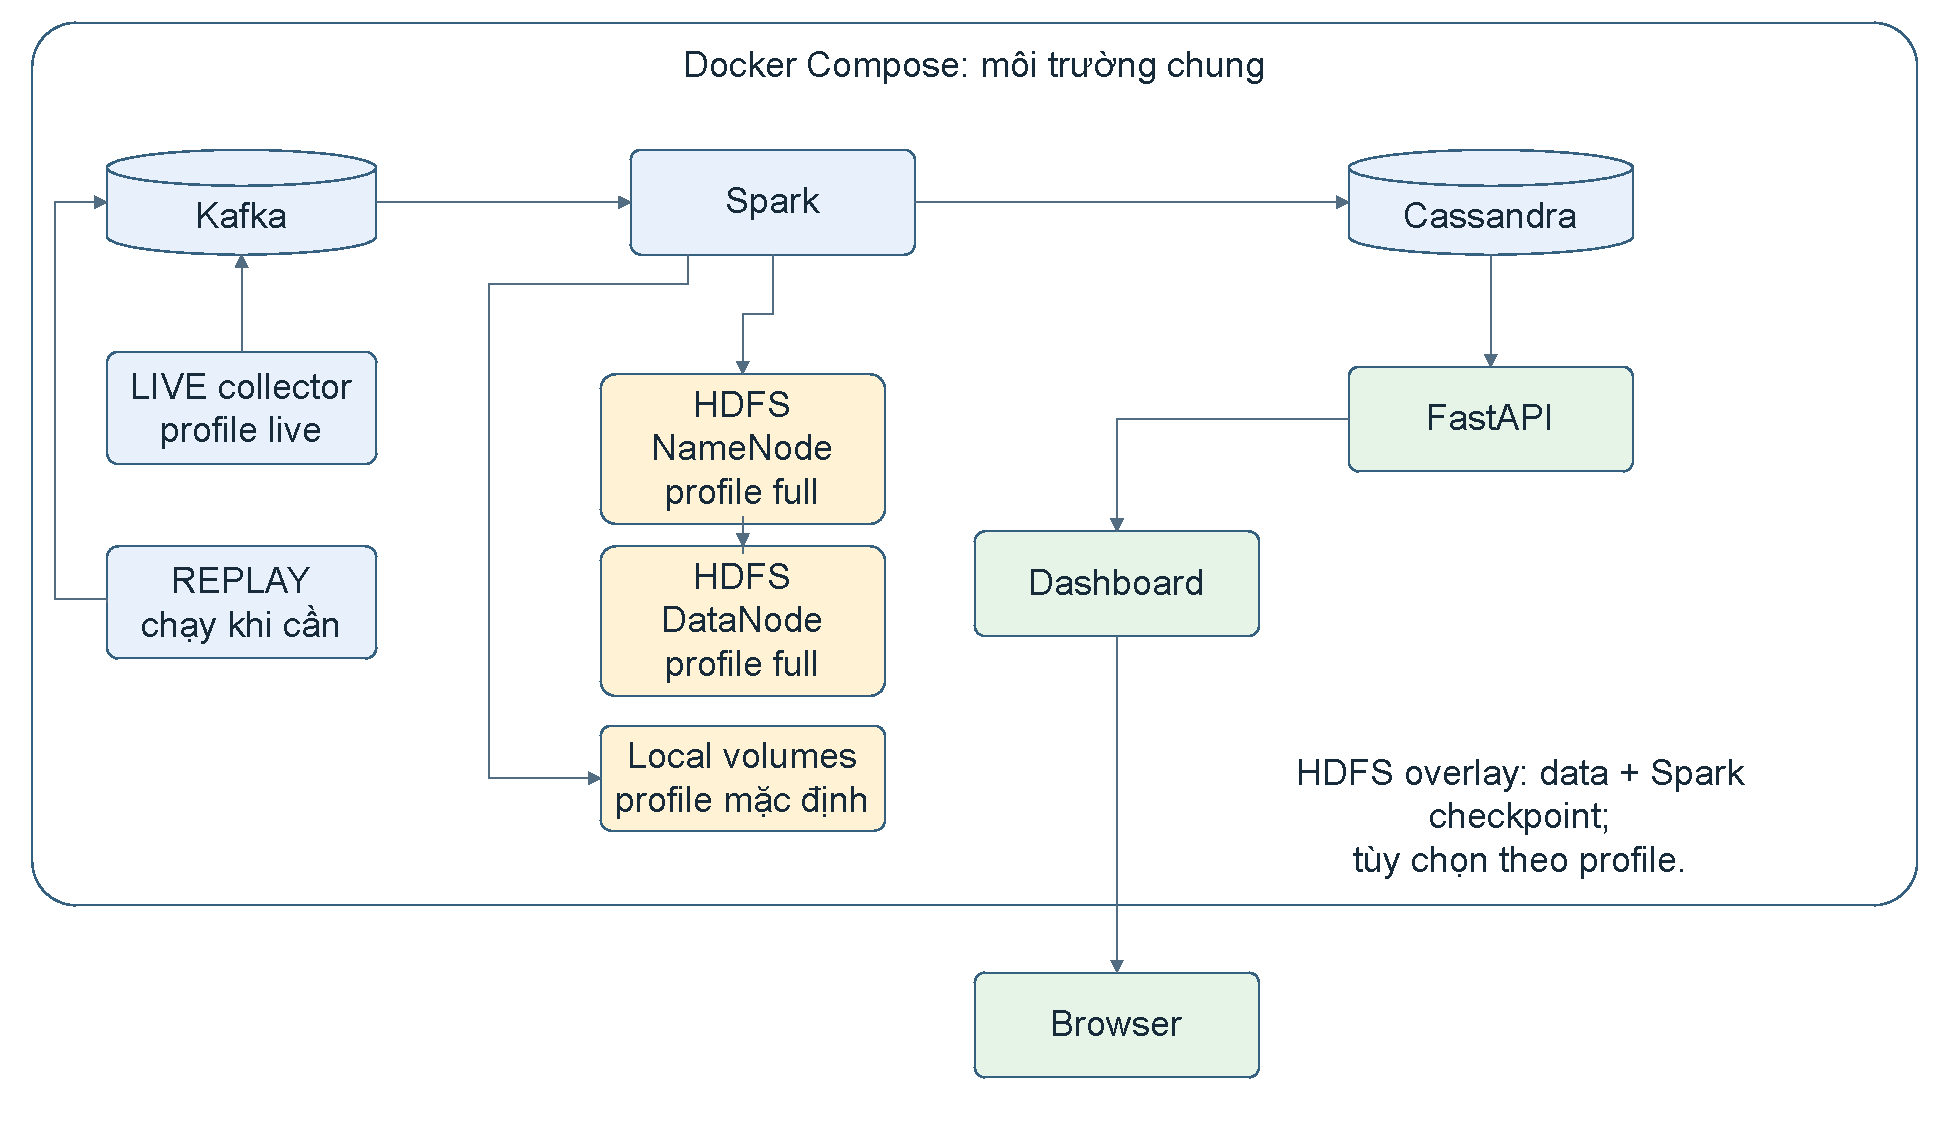
\includegraphics[width=\linewidth,height=0.68\textheight,keepaspectratio]{so-do/design-deployment.pdf}
\caption{Triển khai theo Docker Compose. Profile mặc định dùng local volume; profile full cùng HDFS overlay đưa dữ liệu và checkpoint vào HDFS.}\label{fig:trienkhai}
\end{figure}
Profile \code{full} bổ sung HDFS NameNode/DataNode; overlay HDFS chuyển dữ liệu Parquet và Spark checkpoint sang HDFS.
Profile mặc định dùng local volume. Kubernetes và monitoring mới có skeleton; không xem chúng là triển khai production.
\dukiensua{Trọng review hình triển khai và cấu hình profile.}

\section{Đường đi của một sự kiện}
Hình~\ref{fig:hoatdong} minh họa các bước kiểm tra trước khi một sự kiện được đếm. Bronze raw ghi các bản ghi Kafka mà query tương ứng đã đọc; các query là độc lập và không bảo đảm mọi sự kiện nguồn luôn được lưu.

\begin{figure}[H]
\centering
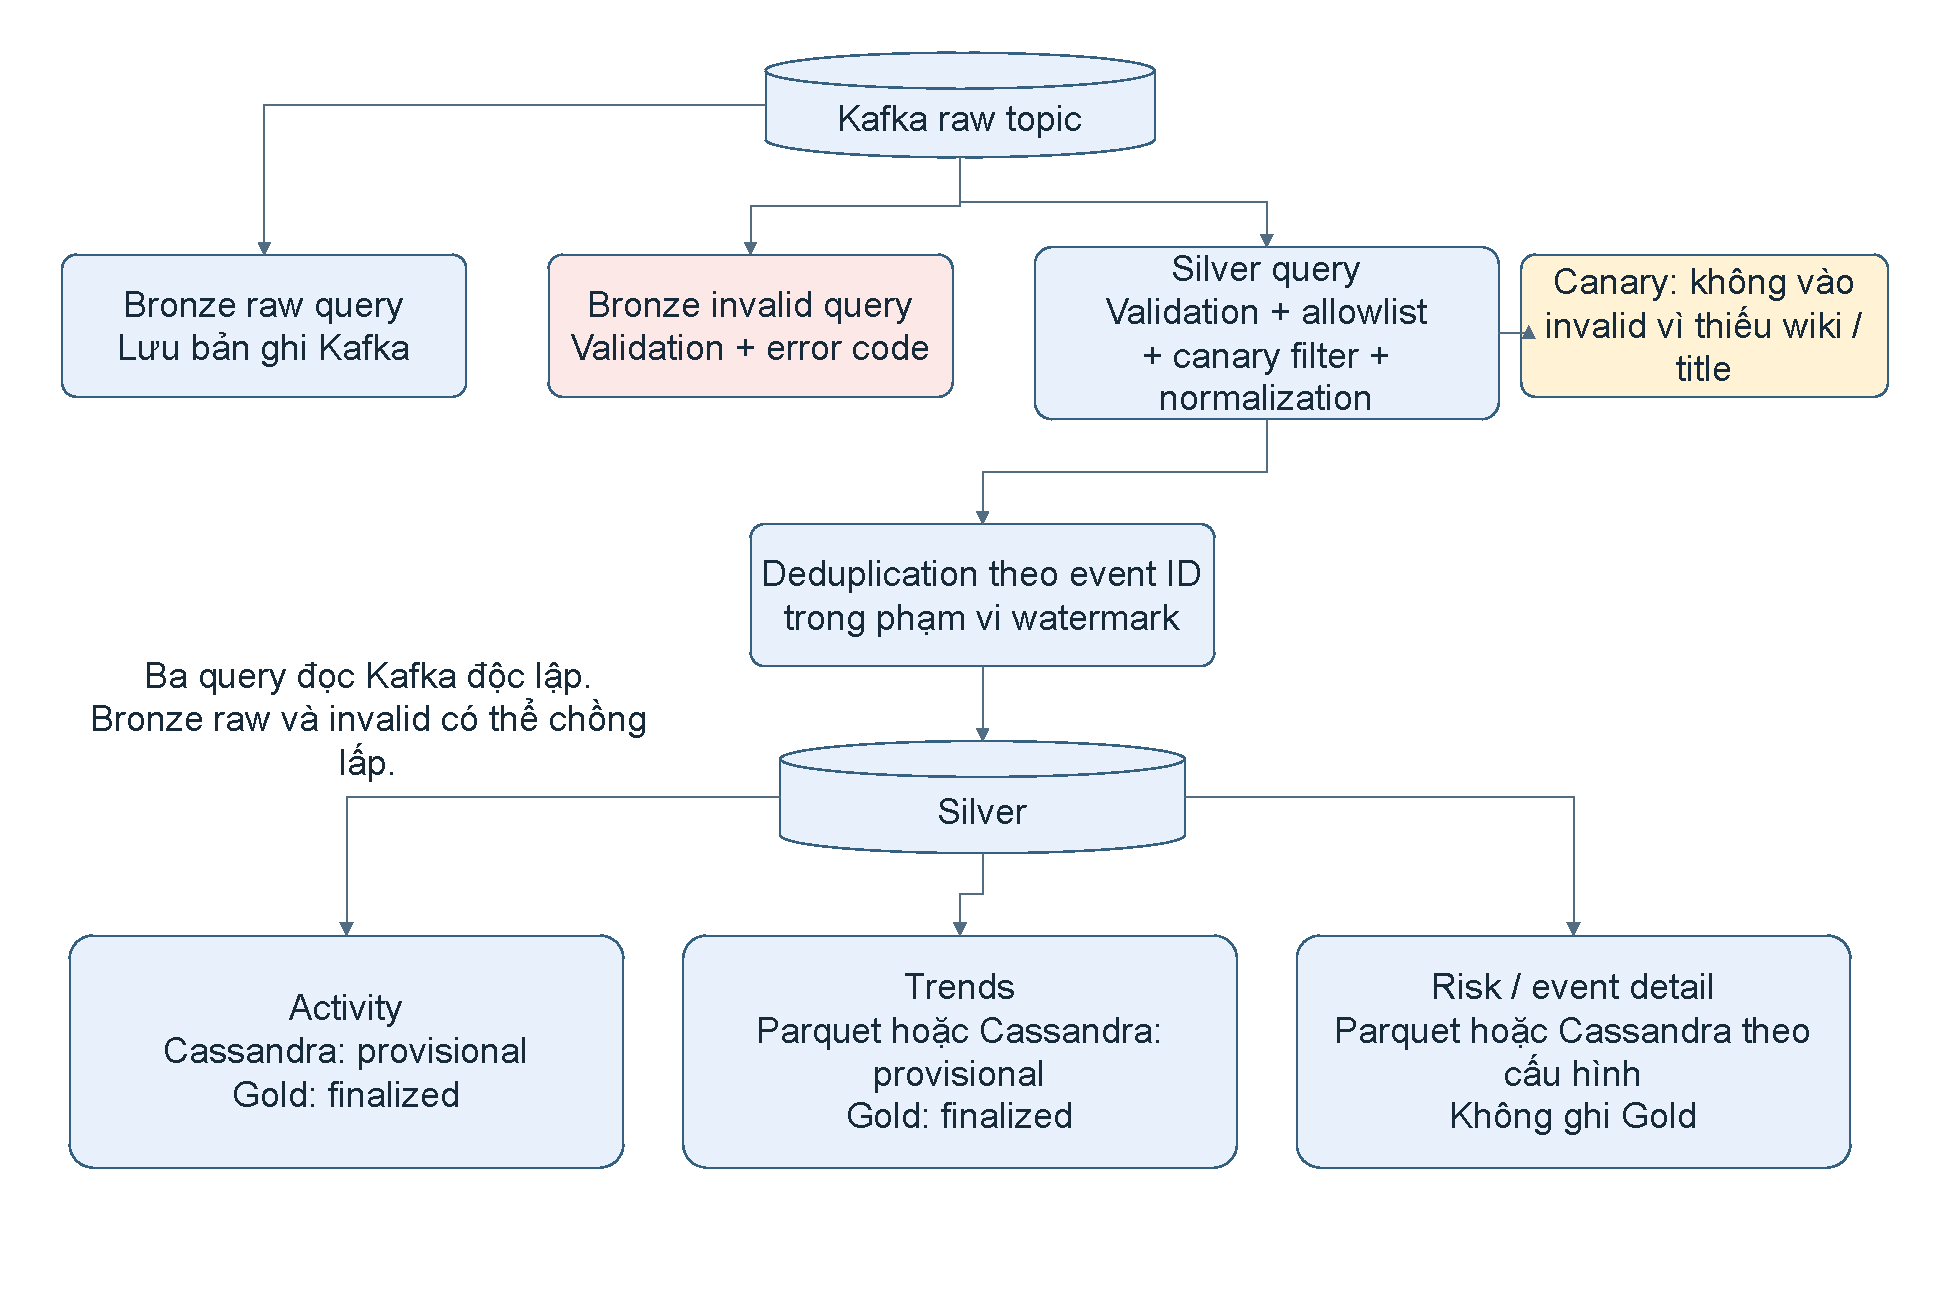
\includegraphics[width=\linewidth,height=0.68\textheight,keepaspectratio]{so-do/design-event-flow.pdf}
\caption{Các query đọc Kafka độc lập. Bronze raw và Bronze invalid có thể chồng lấp; Silver lọc canary và allowlist trước deduplication.}\label{fig:hoatdong}
\end{figure}

\section{Biểu đồ tuần tự: người xem mở trang Overview}\chualam
\dukiensua{Vẽ sau khi W1-MANH-01 xong, lúc luồng dashboard $\rightarrow$ API $\rightarrow$ Cassandra đã ổn định.}

\section{Cấu hình và tách lần chạy}
Mọi tham số (chế độ LIVE hay REPLAY, danh sách wiki, độ trễ watermark, địa chỉ các dịch vụ\ldots) được đọc từ biến môi
trường và kiểm tra ngay khi khởi động, trước khi mở kết nối tốn tài nguyên. Mỗi lần chạy có một \textbf{mã lần chạy};
dữ liệu và checkpoint của lần chạy nằm trong thư mục riêng mang mã đó, và mỗi truy vấn Spark có checkpoint riêng. Khi đổi
schema hay nguồn dữ liệu, nhóm tạo mã lần chạy và keyspace Cassandra mới chứ không xóa checkpoint rồi ghi tiếp vào kết quả
cũ. Kiểm thử end-to-end dùng mã lần chạy và vùng lưu trữ riêng nên không đụng dữ liệu đang dùng để phát triển.

\section{Thu thập dữ liệu}
\subsection{Kafka}
Hệ thống tạo ba topic cho raw, dead-letter queue (DLQ) và pipeline alerts; raw có ba partition, cấu hình demo có một
broker và replication factor 1. Topic DLQ đã tạo nhưng cách dùng Kafka DLQ sink còn chờ nhóm thống nhất; Bronze invalid
hiện lưu bản ghi lỗi. Với JSON object, envelope giữ trường nguồn và thêm \code{ingested\_at}, \code{collector\_version};
key là wiki và page ID, thiếu page ID thì dùng title. JSON sai hoặc không phải object được gửi nguyên văn không key.

\subsection{Phát lại dữ liệu mẫu}
Bộ phát lại đọc file dữ liệu mẫu và gửi từng dòng vào Kafka, giữ nguyên định danh và thời điểm sự kiện; tham số tốc độ
chỉ đổi nhịp gửi. Dữ liệu mẫu ngày 01/01/2026 có 11 dòng, được chọn để thử đủ các nhánh ở Hình~\ref{fig:hoatdong}: 5
chỉnh sửa enwiki, 1 trang mới viwiki, 1 bản trùng, 2 bản hỏng, 1 sự kiện canary, và 1 sự kiện lúc 00:12:10 để đẩy
watermark qua cửa sổ 00:00 (Hình~\ref{fig:watermark}).

Replay có thể dùng khoảng nghỉ cố định hoặc \code{original timing}. Với chế độ thứ hai, khoảng nghỉ dựa vào chênh lệch
event time hợp lệ và speed; event time và ID gốc không bị đổi. Dòng trống được bỏ qua, lỗi gửi làm lượt replay dừng.

\subsection{Thu thập luồng thật}
Collector đọc SSE từ Wikimedia, đóng gói sự kiện rồi gửi Kafka. Các ACK có thể về khác thứ tự; collector chỉ tiến
cursor sau chuỗi ACK thành công liên tiếp. Khi SSE ngắt, collector reconnect với backoff và dùng cursor hiện có làm
\code{Last-Event-ID}. Các event gần lỗi có thể được gửi lại; việc restart process không khôi phục cursor. Vì vậy không
cam kết exactly-once hoặc không mất sự kiện trong mọi tình huống.

\begin{figure}[H]
\centering
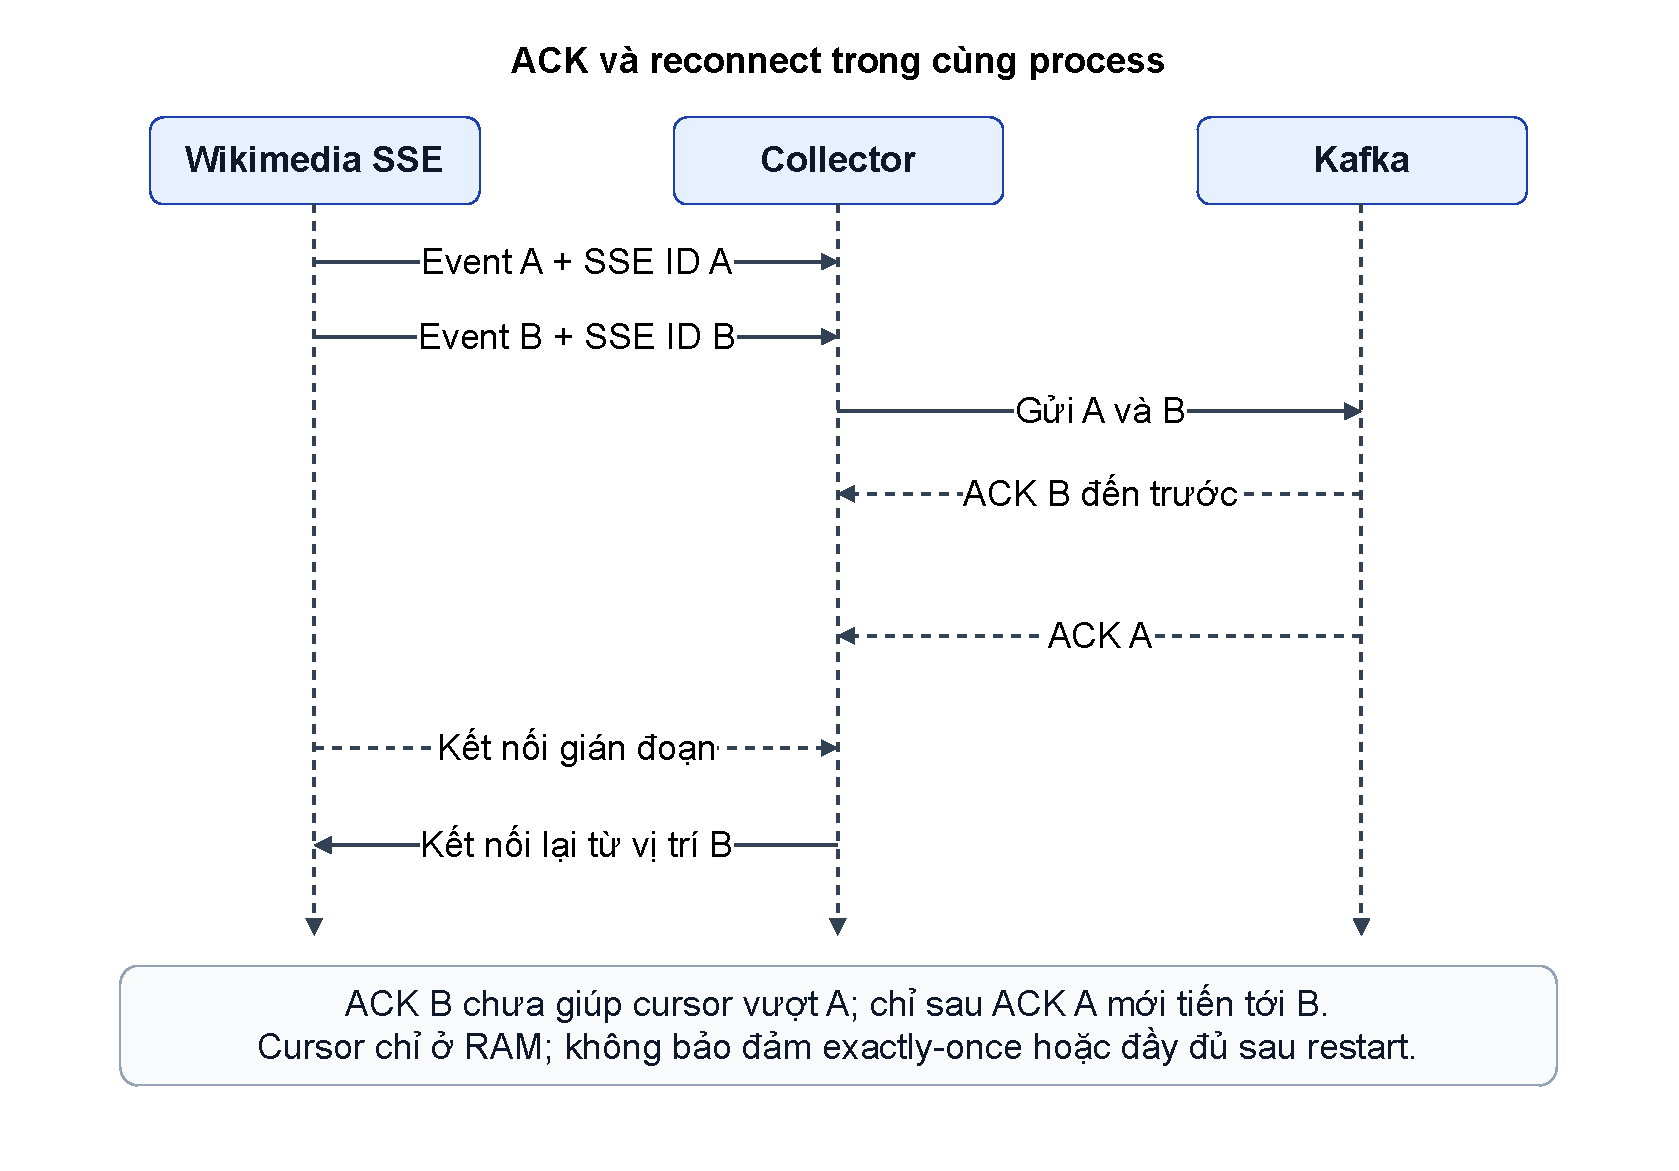
\includegraphics[width=\linewidth,height=0.55\textheight,keepaspectratio]{so-do/seq-ack.pdf}
\caption{ACK và reconnect: cursor chỉ tồn tại trong bộ nhớ process; hình không bảo đảm không mất hoặc không trùng sự kiện.}\label{fig:ack-reconnect}
\end{figure}

Recording là lựa chọn cục bộ: sau ACK liên tiếp, collector ghi bản sao chọn lọc, thay user bằng mã giả và loại comment
nguồn, chỉ giữ nhãn hoàn tác theo heuristic. Title và metadata vẫn có thể chứa danh tính; recording không phải anonymous
hoàn toàn và không được commit nguyên trạng. LIVE raw trong Kafka/Bronze vẫn có thể chứa user hoặc IP từ nguồn.
\dukiensua{Thành và Linh review mô tả collector/contract; nghiệm thu LIVE end-to-end còn chờ nhóm.}

\section{Xử lý luồng}\label{sec:spark}
\subsection{Các truy vấn}
Một tiến trình Spark chạy chín query độc lập trong cấu hình analytics, mỗi query có checkpoint riêng
(Bảng~\ref{tab:truyvan}). Silver được lưu trước khi các query đếm và analytics đọc lại. Cách này tách deduplication
khỏi aggregation và giúp khôi phục từng query theo checkpoint.

\begin{table}[H]
\centering\small
\caption{Các truy vấn streaming}\label{tab:truyvan}
\begin{tabularx}{\linewidth}{@{}lXl@{}}
\toprule
\textbf{Truy vấn} & \textbf{Việc làm} & \textbf{Ghi vào (chế độ)} \\ \midrule
Bronze thô & Đọc Kafka, giữ nguyên bản ghi và vị trí trong Kafka & Parquet (append) \\
Bronze hỏng & Đọc Kafka, lọc bản ghi hỏng, gắn mã lỗi & Parquet (append) \\
Silver & Đọc Kafka, lọc, chuẩn hóa, loại trùng & Parquet (append) \\
Hoạt động tạm tính & Đọc Silver, đếm theo wiki và phút & Cassandra (update) \\
Hoạt động đã chốt & Đọc Silver, đếm như trên & Parquet Gold (append) \\
Trends provisional & Đọc Silver, tính xu hướng theo window & Parquet hoặc Cassandra (update) \\
Suspicious edits & Đọc Silver, chọn edit có risk score lớn hơn 0 & Parquet hoặc Cassandra (append) \\
Event details & Đọc Silver, tạo chi tiết sự kiện & Parquet hoặc Cassandra (append) \\
Trends finalized & Đọc Silver, tính xu hướng đã chốt & Parquet Gold (append) \\
\bottomrule
\end{tabularx}
\end{table}

\subsection{Event ID và deduplication}
Định danh của sự kiện lấy từ nguồn. Nếu nguồn không có, hệ thống tự tạo bằng cách băm các trường không đổi của sự kiện
(wiki, trang, phiên bản, thời điểm, loại); không bao giờ dùng thời điểm nhận hay xử lý, vì như vậy cùng một sự kiện gửi
hai lần sẽ có hai định danh khác nhau. Mọi phép biến đổi dùng hàm có sẵn của Spark, không viết hàm Python riêng, để Spark
tối ưu được và không phải chuyển dữ liệu qua lại giữa Java và Python.

\subsection{Đếm hoạt động}
Với mỗi wiki và mỗi phút, hệ thống đếm: tổng sự kiện hợp lệ, số chỉnh sửa, số trang mới, và trong số chỉnh sửa thì bao
nhiêu là ẩn danh, bao nhiêu là của bot.

\subsection{Đặc trưng xu hướng}
Với từng wiki và trang, Spark tính trên window 5 phút trượt mỗi phút: số edit, số editor ước lượng bằng
\code{approx\_count\_distinct} trên user hash, và tổng độ lớn byte delta. Trend score kết hợp ba đặc trưng sau chuẩn hóa
và giới hạn theo cấu hình. Metadata của trang được chọn theo thứ tự ổn định của event time, event ID, title, namespace,
không theo thứ tự nhận. Kết quả provisional có thể thay đổi; Gold finalized được ghi khi watermark cho phép.

\subsection{Chấm điểm ưu tiên xem xét}
Risk score chỉ áp dụng cho event type edit. Cấu hình mặc định cộng 30 điểm khi xóa ít nhất 500 byte, 20 điểm khi comment
khớp heuristic revert tiếng Anh và 10 điểm cho anonymous edit không phải bot; tổng bị chặn theo mức cấu hình. Một edit
có thể khớp nhiều dấu hiệu. Điểm này hỗ trợ ưu tiên xem xét, không kết luận chỉnh sửa là phá hoại.
\dukiensua{Linh review mô tả scoring, watermark và ví dụ fixture trước khi chốt báo cáo.}

\section{Lưu trữ}
\subsection{Tầng Parquet}
Bronze và Silver chia thư mục theo ngày và giờ của sự kiện; Gold chia theo ngày, giờ và wiki. Danh sách đầy đủ các trường
của Silver nằm trong tài liệu contract của nhóm.
Parquet có thể lưu trên local volume hoặc HDFS theo cấu hình; các query dùng checkpoint riêng. Bài thử HDFS và phục hồi
trên fixture được trình bày ở chương kiểm thử, không mặc định đại diện cho tải production.

\subsection{Lược đồ Cassandra}\label{sec:cassandra}
Bảng hoạt động theo cửa sổ (Hình~\ref{fig:bangcass}) phục vụ đúng hai câu hỏi của API: \enquote{các phút mới nhất của
một wiki} và \enquote{một phút cụ thể của một wiki}. Cách chọn khóa đã giải thích ở Hình~\ref{fig:cassandra}.

\begin{figure}[H]
\centering
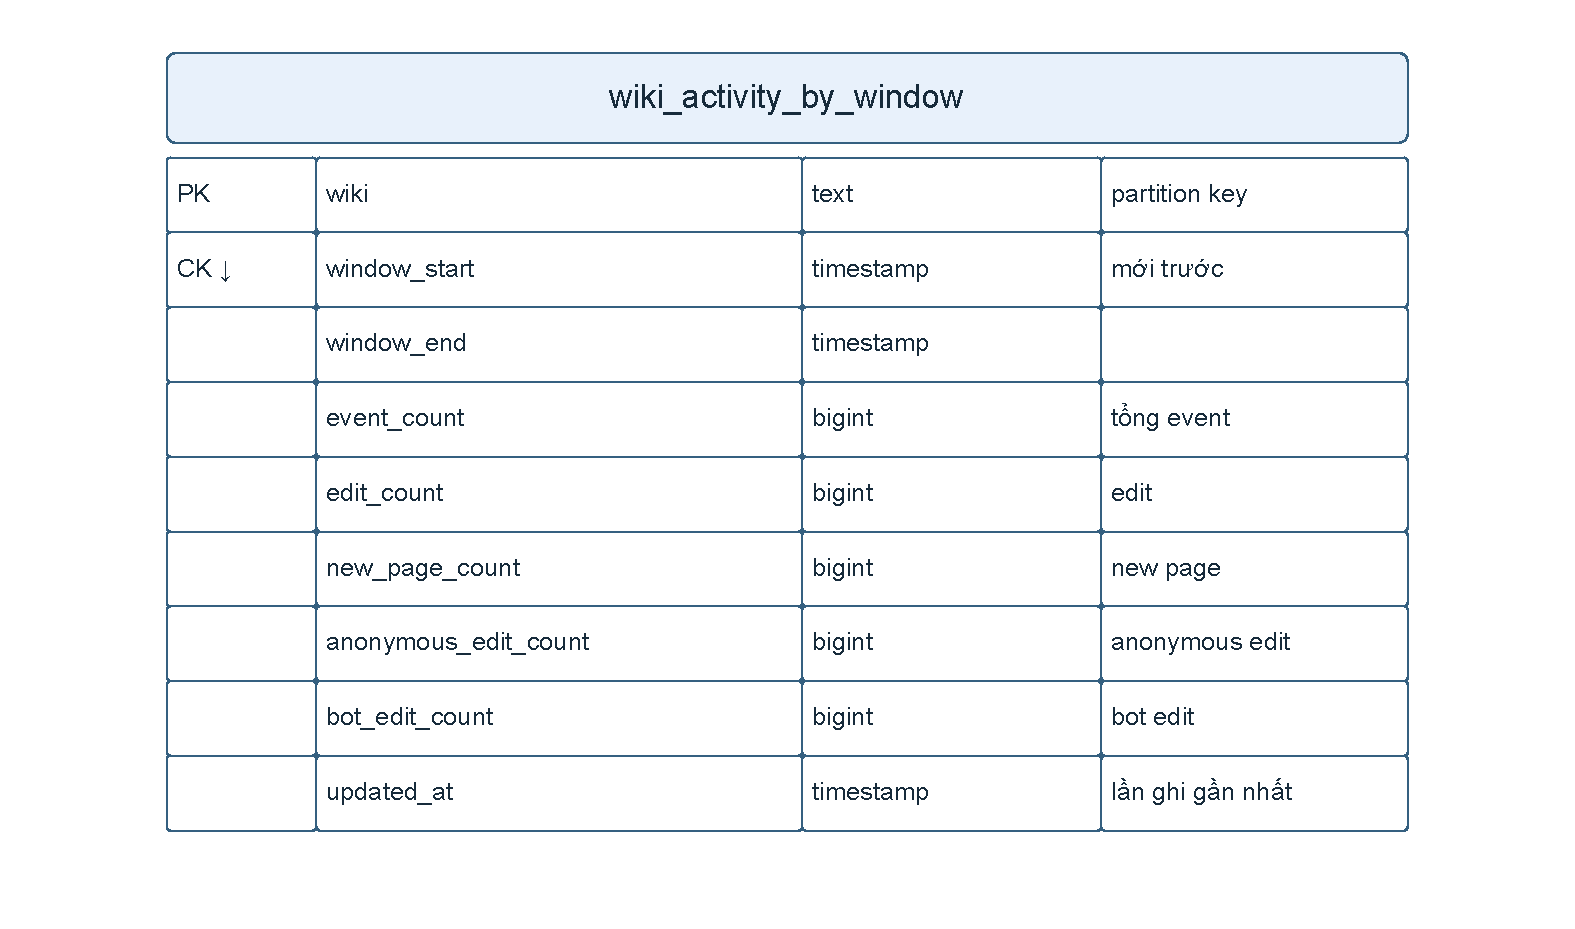
\includegraphics[width=\linewidth,height=0.68\textheight,keepaspectratio]{so-do/design-cassandra-activity.pdf}
\caption{Bảng hoạt động theo cửa sổ. PK: khóa partition; CK$\downarrow$: khóa sắp xếp, giảm dần.}\label{fig:bangcass}
\end{figure}

\begin{itemize}
  \item Spark ghi \textbf{tổng số} của cửa sổ, không ghi phần cộng thêm, nên ghi lại sau sự cố không làm đếm đôi.
  \item Mỗi wiki thêm 1.440 dòng mỗi ngày, khoảng 525 nghìn dòng mỗi năm: đủ cho demo. Trước khi chạy LIVE dài ngày cần
        đặt thời hạn tự xóa (TTL) hoặc chia partition theo ngày.
  \item Trước khi ghi, mỗi dòng được kiểm tra: tên wiki hợp lệ, cửa sổ kết thúc sau khi bắt đầu, số đếm nhất quán (chỉnh
        sửa cộng trang mới không vượt tổng; ẩn danh, bot không vượt số chỉnh sửa). Dòng sai làm batch thất bại;
        batch có thể được replay khi query/process được khởi động lại với checkpoint phù hợp.
\end{itemize}

Ba nghiệp vụ còn lại dùng năm bảng (Hình~\ref{fig:bangw2}). Mỗi query Cassandra cung cấp partition key; một API request
có thể đọc chỉ mục rồi truy vấn một hoặc nhiều partition, tùy nghiệp vụ. Các query không dùng \code{ALLOW FILTERING}.

\begin{figure}[H]
\centering
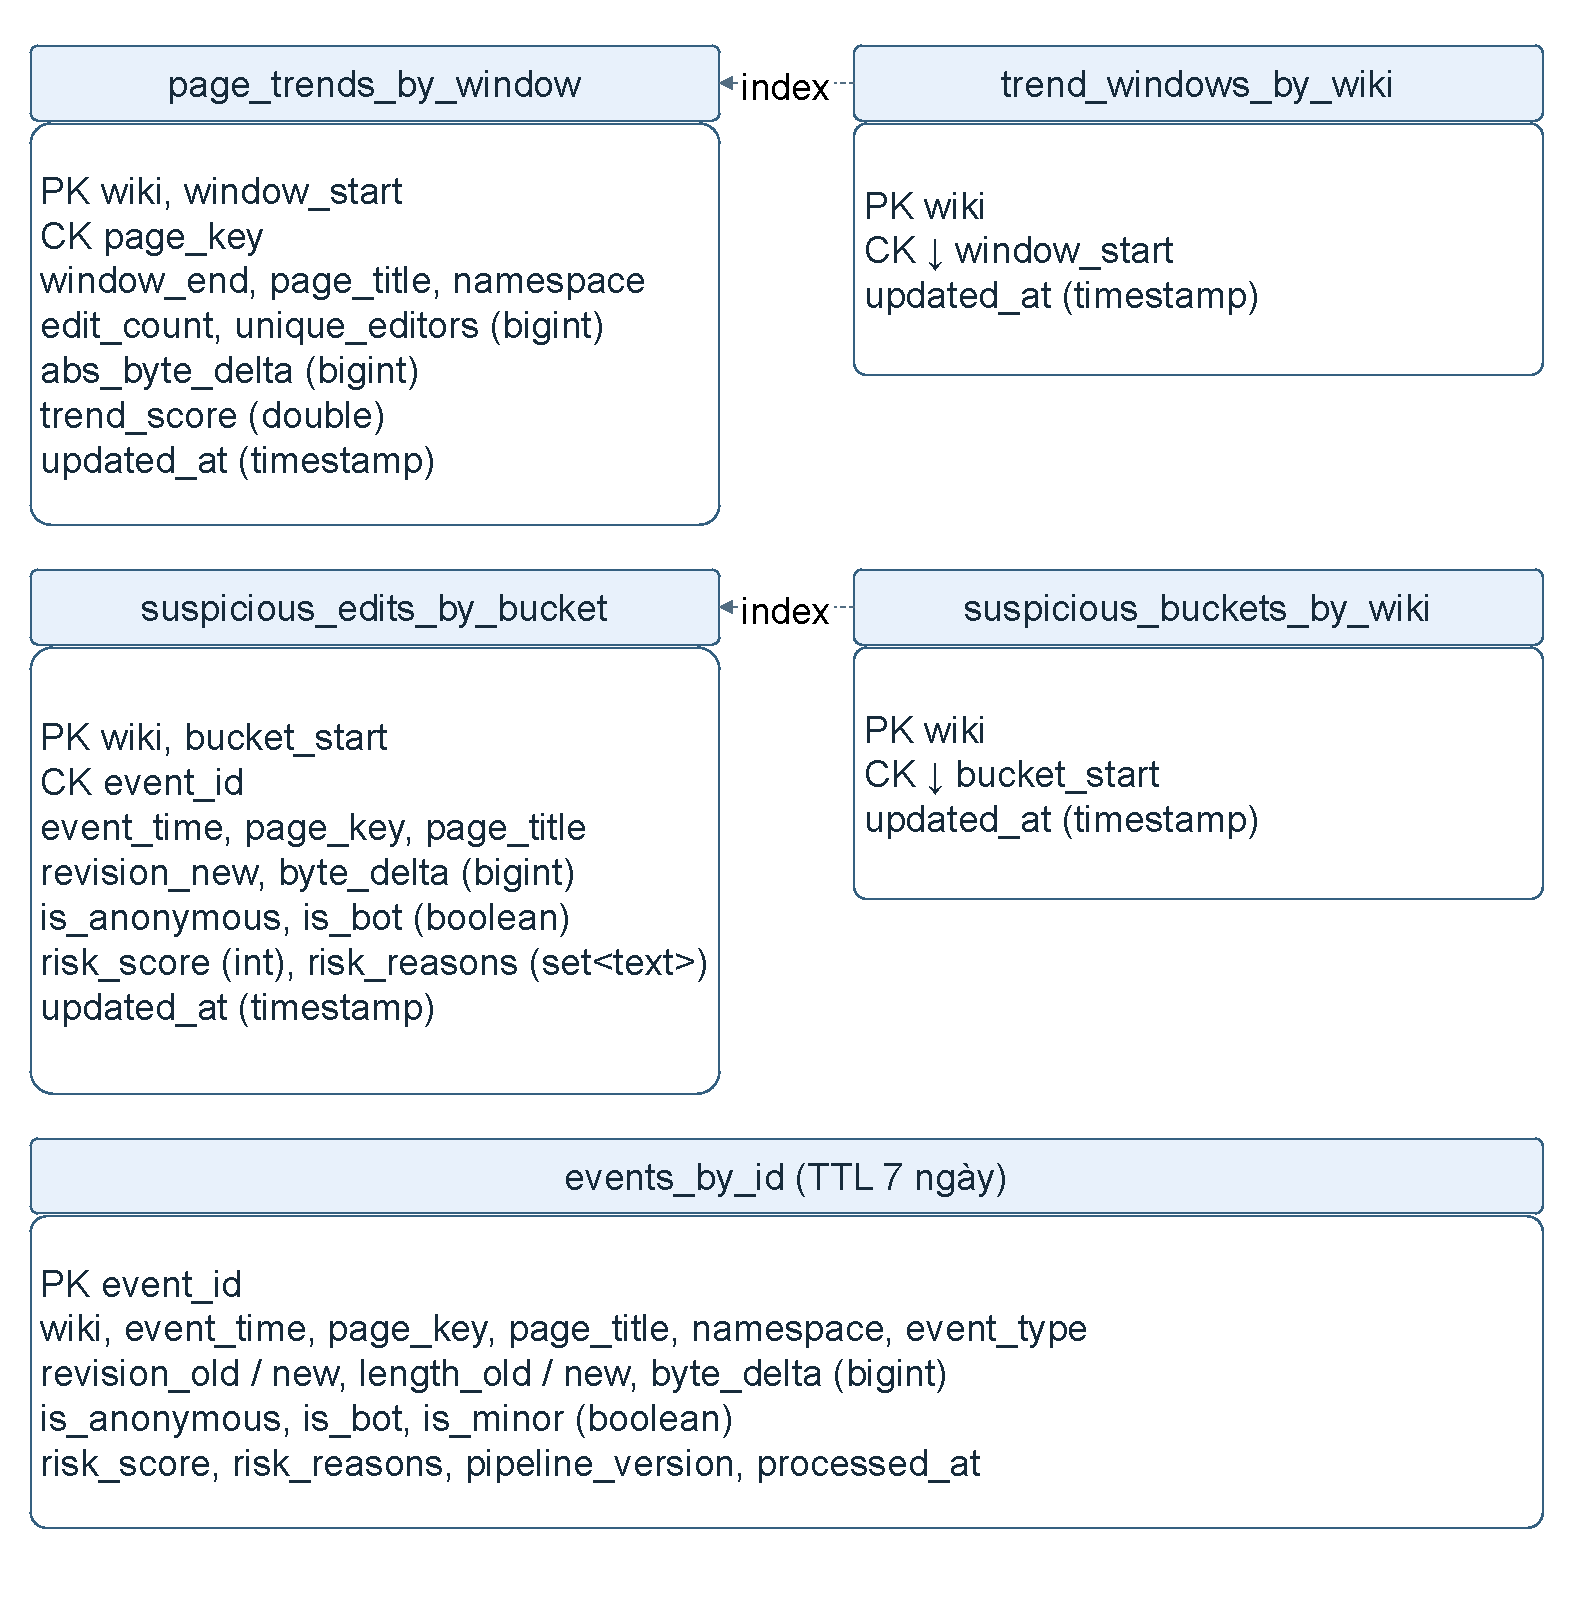
\includegraphics[width=\linewidth,height=0.68\textheight,keepaspectratio]{so-do/design-cassandra-analytics.pdf}
\caption{Năm bảng cho xu hướng, chỉnh sửa cần ưu tiên và chi tiết sự kiện. PK: khóa partition; CK: khóa sắp xếp
($\downarrow$ là giảm dần). Mũi tên nét đứt: bảng chỉ mục liệt kê các cửa sổ (hoặc phút) đã có dữ liệu ở bảng chính.}
\label{fig:bangw2}
\end{figure}

\begin{itemize}
  \item \textbf{Bảng chỉ mục thay cho quét bảng.} Cassandra không trả lời được \enquote{cửa sổ mới nhất của enwiki là cửa
        sổ nào} nếu chỉ có bảng chính, vì khóa partition gồm cả wiki lẫn mốc thời gian. Mỗi wiki vì vậy có thêm một
        partition liệt kê các cửa sổ (hoặc các phút) đã có dữ liệu, mới nhất trước.
  \item \textbf{Thứ tự ghi.} Trong mỗi batch, các dòng dữ liệu được ghi trước, chỉ mục ghi sau. Người đọc thấy một cửa sổ
        trong chỉ mục thì chắc chắn dữ liệu của cửa sổ đó đã có; batch hỏng giữa chừng và được chạy lại cũng chỉ ghi
        đè cùng các khóa.
  \item \textbf{Điểm không nằm trong khóa.} Điểm xu hướng và điểm ưu tiên thay đổi theo từng batch. Nếu đưa điểm vào khóa,
        mỗi lần điểm đổi sẽ sinh ra một dòng mới và dòng cũ vẫn còn. Vì vậy API đọc cả partition rồi tự sắp xếp.
  \item \textbf{Giới hạn 5.000 dòng.} Đọc cả partition chỉ an toàn khi partition nhỏ. API đọc tối đa 5.001 dòng; nếu
        thật sự có hơn 5.000 dòng thì báo vượt dung lượng chứ không trả bảng xếp hạng thiếu. Với chỉnh sửa cần ưu tiên,
        giới hạn tính trên tổng số dòng của mọi phút được đọc.
  \item \textbf{Hạn lưu chi tiết sự kiện.} Bảng chi tiết sự kiện tự xóa dòng sau 7 ngày. Lịch sử đầy đủ vẫn nằm ở Bronze
        và Silver; số đo làm căn cứ cho mốc 7 ngày ở Mục~\ref{sec:dungluong}.
  \item \textbf{Kiểm tra trước khi ghi.} Như bảng hoạt động, mỗi dòng phải đúng tập trường của contract (dòng có thêm định
        danh người dùng hay nội dung bình luận bị từ chối), cửa sổ xu hướng dài đúng 5 phút, phút của chỉnh sửa khớp
        thời điểm sự kiện, lý do ưu tiên thuộc ba mã đã định. Chỉ những trường Spark luôn điền mới bị kiểm tra bắt
        buộc, để một trường được phép trống không làm luồng thất bại lặp lại.
\end{itemize}

\subsection{Ghi kết quả từ Spark sang Cassandra}
Ở mỗi batch, tiến trình chính của Spark duyệt lần lượt từng dòng kết quả (không nạp cả batch vào bộ nhớ) và ghi vào
Cassandra. Nếu ghi lỗi, truy vấn dừng; khi query/process được khởi động lại với checkpoint phù hợp, batch có thể được replay. Parquet và Cassandra không có giao dịch
chung, nên hệ thống không cam kết \enquote{đúng một lần} trên cả hai nơi; tính đúng dựa vào việc ghi đè theo khóa ổn định.

\section{API}
\begin{table}[H]
\centering\small
\caption{Các endpoint}\label{tab:api}
\begin{tabularx}{\linewidth}{@{}lXl@{}}
\toprule
\textbf{Endpoint} & \textbf{Mô tả} & \textbf{Trạng thái} \\ \midrule
\code{/health} & Kiểm tra Cassandra thật sự trả lời được & Đã làm \\
\code{/api/v1/activity} & Hoạt động theo cửa sổ; chọn wiki, một cửa sổ cụ thể, số dòng tối đa 100 & Đã làm \\
\code{/api/v1/trends} & Top-N trang xu hướng của một cửa sổ 5 phút (mặc định cửa sổ mới nhất) & Đã làm \\
\code{/api/v1/suspicious-edits} & Chỉnh sửa cần ưu tiên trong 1--15 phút gần nhất, lọc theo điểm tối thiểu & Đã làm \\
\code{/api/v1/events/\{id\}} & Chi tiết một sự kiện & Đã làm \\
\bottomrule
\end{tabularx}
\end{table}

Các phản hồi dữ liệu kèm thời điểm tạo, nguồn và chế độ chạy; activity, trends và suspicious edits có nhãn \code{provisional}, còn event detail không có trường này. Mọi thời điểm theo UTC. Danh sách
không có dữ liệu được trả rỗng; event ID không tìm thấy trả 404. Tham số sai (wiki ngoài danh sách, cửa sổ thiếu múi giờ, số dòng ngoài
1--100) bị từ chối. Cassandra không trả lời thì API báo \enquote{phụ thuộc chưa sẵn sàng}; API vẫn khởi động được khi
Cassandra chưa lên và tự hồi phục khi Cassandra sẵn sàng. Danh sách chỉnh sửa cần ưu tiên luôn kèm câu nhắc điểm chỉ
để ưu tiên xem xét. API không trả các trường user, IP, comment hoặc user hash; page title vẫn có thể chứa thông tin nhận dạng.

Mọi lỗi có cùng một dạng: một mã lỗi cố định để chương trình đọc, một câu mô tả cho người đọc, và thông tin thêm tùy
loại (Bảng~\ref{tab:loi}). Lỗi tham số do thư viện web tự phát hiện (ví dụ số dòng bằng 0) cũng được đổi về dạng này,
để dashboard chỉ cần một cách đọc lỗi.

\begin{table}[H]
\centering\small
\caption{Các loại lỗi của API}\label{tab:loi}
\begin{tabularx}{\linewidth}{@{}llX@{}}
\toprule
\textbf{HTTP} & \textbf{Mã} & \textbf{Khi nào; thông tin thêm} \\ \midrule
422 & \code{INVALID\_QUERY} & Tham số sai; kèm danh sách tham số sai và lý do \\
404 & \code{EVENT\_NOT\_FOUND} & Không có sự kiện với định danh đã cho \\
503 & \code{DEPENDENCY\_UNAVAILABLE} & Cassandra không trả lời; kèm tên dịch vụ lỗi \\
503 & \code{CAPACITY\_EXCEEDED} & Phải đọc hơn 5.000 dòng để trả lời \\
\bottomrule
\end{tabularx}
\end{table}

\section{Dashboard}
Bốn trang: Overview (đọc dữ liệu activity theo wiki và cửa sổ 1 phút, tự làm mới sau 15 giây), Trending (Top-N trang tăng hoạt động trong cửa sổ 5 phút kèm liên kết Wikipedia), Suspicious Edits (danh sách chỉnh sửa ưu tiên xem xét với bộ lọc bot/điểm rủi ro và xem chi tiết sự kiện), và System Status (readiness của API và Cassandra). Giao diện không hiển thị các trường IP, username thô hay \code{user\_hash}; page title vẫn có thể chứa thông tin nhận dạng.
\dukiensua{Mạnh bổ sung ảnh chụp các trang mới (W2-MANH-01) và chuẩn hóa tên file ảnh không dấu/không khoảng trắng.}

% ============================================================================
% CHƯƠNG 5: KIỂM THỬ VÀ ĐÁNH GIÁ
% ============================================================================

\chapter{Kiểm thử và đánh giá}\label{chap:danhgia}

\section{Chiến lược kiểm thử}
\begin{table}[H]
\centering\small
\caption{Các tầng kiểm thử}\label{tab:kiemthu}
\begin{tabularx}{\linewidth}{@{}lXl@{}}
\toprule
\textbf{Tầng} & \textbf{Nội dung} & \textbf{Khi chạy} \\ \midrule
Nhẹ & Cấu hình, API, lớp truy cập Cassandra, phát lại, dashboard; Cassandra được giả lập ở tầng driver nhưng giữ đúng cách ghi đè theo khóa & Mỗi lần sửa code, vài giây \\
Hồi quy contract & Mô tả API công bố phải trùng bản đã lưu; cột của lược đồ Cassandra phải trùng các trường lớp truy cập kiểm tra; từ điển dữ liệu phải liệt kê đủ bảng & Cùng tầng nhẹ \\
Spark & Các phép biến đổi và cách điều phối truy vấn, chạy trong container có Java & Khi sửa phần xử lý \\
Tích hợp & Lớp truy cập trên Cassandra thật, keyspace ngẫu nhiên, tự xóa sau khi chạy & Khi sửa lược đồ, truy vấn \\
End-to-end & Dựng hệ thống riêng, phát dữ liệu mẫu hai pha, kiểm tra cả ba tầng, API và giao diện & Trước khi nghiệm thu \\
\bottomrule
\end{tabularx}
\end{table}
Lệnh chạy từng tầng ở Phụ lục~\ref{app:ma}. Tầng hồi quy contract giúp thay đổi giao diện không lọt qua âm thầm.
Đổi tham số, trường trả về hay cột lưu trữ mà không cập nhật bản mô tả API đã lưu thì test thất bại. Người sửa vì thế
phải cập nhật cả bản mô tả lẫn contract của nhóm trong cùng một lần nộp.

\section{Kết quả CP0}
Dữ liệu mẫu ngày 01/01/2026 gồm 11 bản ghi. Kết quả chạy thật (Bảng~\ref{tab:cp0}) khớp bộ kết quả kỳ vọng; bộ này
được viết tay độc lập, không sinh ra từ chính code xử lý.

\begin{table}[H]
\centering\small
\caption{Kết quả CP0 trên dữ liệu mẫu, cửa sổ 2026-01-01 00:00 UTC}\label{tab:cp0}
\begin{tabularx}{\linewidth}{@{}Xr@{}}
\toprule
\textbf{Chỉ tiêu} & \textbf{Kết quả} \\ \midrule
Bản ghi Kafka / Bronze raw & 11 / 11 \\
Bronze invalid & 2 \\
Silver (sau loại trùng và canary) & 7 \\
Gold cửa sổ 00:00 (đã chốt) & 2 dòng \\
enwiki: event / edit / trang mới / ẩn danh / bot & 5 / 5 / 0 / 1 / 1 \\
viwiki: event / edit / trang mới / ẩn danh / bot & 1 / 0 / 1 / 0 / 0 \\
\bottomrule
\end{tabularx}
\end{table}

\begin{table}[H]
\centering\small
\caption{Các lần kiểm chứng}\label{tab:kiemchung}
\begin{tabularx}{\linewidth}{@{}llX@{}}
\toprule
\textbf{Ngày} & \textbf{Máy} & \textbf{Kết quả} \\ \midrule
11/10/2026 & Apple M3, ARM64 & 84 test nhẹ đạt; 16 test Spark đạt; kiểm thử end-to-end đạt (Trọng) \\
15/10/2026 & Windows 11, x86\_64 & CP0 chạy lại, số khớp Bảng~\ref{tab:cp0} (Thành) \\
22/10/2026 & Windows 11, x86\_64 & Bộ \code{api/tests} đạt 33 test; lượt Cassandra integration đạt 4 test (Nhân) \\
23/11/2026 & Windows 11, x86\_64 & 179 test nhẹ toàn repo, gồm 68 test API; một lượt riêng có 8 test Cassandra thật đạt; end-to-end ghi Cassandra khớp Bảng~\ref{tab:w2fixture} (Nhân) \\
23/11/2026 & Windows 11, x86\_64 & Hồi quy sau khi gộp: 183 test nhẹ đạt (gồm 4 test hồi quy contract); 8 test trên Cassandra thật đạt; kiểm thử end-to-end đạt; các lệnh vận hành serving chạy đúng trên hệ thống thật (Nhân) \\
\bottomrule
\end{tabularx}
\end{table}
\dukiensua{Mỗi thành viên chạy lại CP0 trên máy mình thì thêm một dòng (CP1).}

\begin{ghichu}{Bài học khi chạy trên Windows}
Hai lỗi chỉ xuất hiện trên Windows. (1) Git trên Windows mặc định đổi ký tự xuống dòng của file sang kiểu Windows (CRLF);
script tạo topic chạy trong container Linux vì thế đọc sai và dừng. Cách sửa: khai báo cho Git luôn giữ kiểu Linux (LF)
với mọi script shell. (2) Thư viện Cassandra cho Python cần một module đã bị gỡ khỏi Python 3.12; container dùng
Python 3.11 nên không bị, còn máy phát triển dùng 3.12 phải cài thêm gói thay thế. Bài học: mỗi thành viên nên chạy lại
toàn bộ hệ thống trên máy mình sớm (mốc CP1), vì lỗi môi trường không lộ ra khi chỉ chạy trên một máy.
\end{ghichu}

\section{Xu hướng và ưu tiên xem xét trên fixture vàng}
Ngày 23/11/2026, nhóm dựng một hệ thống riêng với Spark ghi cả ba nghiệp vụ mới vào Cassandra, phát lại toàn bộ 11 bản ghi
mẫu rồi hỏi qua API. Cả chín truy vấn Spark đều chạy. Mọi số liệu API trả về (Bảng~\ref{tab:w2fixture}) trùng với bộ
kỳ vọng viết tay độc lập mà phần xử lý dùng để kiểm tra đầu ra Parquet. Như vậy cùng một kết quả đi qua được cả hai
đường lưu: Parquet và Cassandra.

\begin{table}[H]
\centering\small
\caption{Kết quả qua API trên dữ liệu mẫu (enwiki)}\label{tab:w2fixture}
\begin{tabularx}{\linewidth}{@{}Xr@{}}
\toprule
\textbf{Chỉ tiêu} & \textbf{Kết quả} \\ \midrule
Chi tiết sự kiện lưu trong Cassandra & 7 (bằng số sự kiện Silver) \\
Cửa sổ 00:00--00:05, trang 10: chỉnh sửa / người sửa / byte thay đổi / điểm & 4 / 3 / 1.890 / 0,12475 \\
Cửa sổ 00:00--00:05, trang 11: chỉnh sửa / người sửa / byte thay đổi / điểm & 1 / 1 / 5 / 0,022625 \\
Chỉnh sửa cần ưu tiên: xóa nhiều nội dung / hoàn tác / sửa ẩn danh & điểm 30 / 20 / 10 \\
Sự kiện không dính dấu hiệu nào & điểm 0, không có lý do \\
Định danh không tồn tại & lỗi \enquote{không tìm thấy sự kiện} \\
\bottomrule
\end{tabularx}
\end{table}
Các số trong bảng là kết quả API của cửa sổ provisional 00:00--00:05 ở lần chạy của Nhân. Ở một phép kiểm khác,
Linh ghi nhận Gold finalized cho cửa sổ 23:56--00:01 của ngày hôm trước, với cùng các giá trị trend score trên fixture;
hai kết quả thuộc hai đầu ra và hai cửa sổ khác nhau. Giá trị số người sửa dùng phép ước lượng
\code{approx\_count\_distinct}, không phải cam kết đếm chính xác cho mọi tập dữ liệu.
\dukiensua{Thêm ảnh chụp trang Trending, Suspicious Edits khi W2-MANH-01 xong.}

\section{Độ trễ end-to-end}\chualam
\section{Khởi động lại, retry và dữ liệu đến muộn}
Retry được kiểm tra cho cả bốn loại dữ liệu phục vụ: hoạt động và xu hướng trên Cassandra thật (keyspace tạm, xóa sau
khi chạy), chỉnh sửa cần ưu tiên và chi tiết sự kiện trên bản giả lập ở tầng driver vốn giữ đúng cách ghi đè theo khóa.
Ghi cùng một dòng hai lần, rồi ghi lại với giá trị mới, thì mỗi khóa vẫn chỉ có một dòng mang giá trị mới nhất. Ghi lại các
batch xu hướng không tạo thêm cửa sổ trong chỉ mục. \enquote{Cửa sổ mới nhất} lấy từ chỉ mục luôn là cửa sổ vừa ghi.
Danh sách lý do rỗng đọc ra đúng là rỗng, không thành giá trị trống. Truy vấn theo khoảng phút chạy được mà không cần
cho phép quét bảng.
Lượt kiểm thử W3 của Linh ngày 08/11/2026 dùng Kafka, Spark, HDFS và Cassandra activity trong môi trường cô lập.
Fixture lần lượt đưa duplicate, late event, event làm watermark tiến và event quá muộn vào hệ thống. Bảy trong bảy
phase đạt, chín Spark query giữ query ID qua JVM mới nhờ checkpoint. Đầu ra cuối gồm 13 Bronze raw, 2 Bronze invalid,
6 Silver, 2 suspicious edit, 2 dòng Gold activity và 10 dòng Gold trends. Bronze raw và invalid là hai nhánh
có thể chồng lấp nên không cộng số dòng của chúng thành tổng. Gold được quan sát sau khi event time tiến watermark,
không kết luận rằng chỉ chờ thời gian thực là đủ chốt cửa sổ. Analytics trong lượt này ghi Parquet; kết quả không
chứng minh LIVE end-to-end hoặc exactly-once giữa các sink. Nguồn: \code{docs/plans/W3-LINH-01.md}.

Trong phép thử W3 của Trọng, hệ thống lưu kết quả REPLAY, dừng Spark rồi tạo lại Kafka, Cassandra và HDFS với volume
cũ. API đọc activity khi Spark vẫn dừng, sau đó Spark được khởi động lại từ checkpoint. Trình tự này giúp phân biệt
dữ liệu Cassandra đã còn qua restart với dữ liệu có thể được Spark ghi lại sau restart. Phép thử thuộc REPLAY và
cấu hình riêng được ghi tại \code{docs/plans/W3-TRONG-01.md}; không suy ra mọi kịch bản lỗi đều được bao phủ.

\begin{figure}[H]
\centering
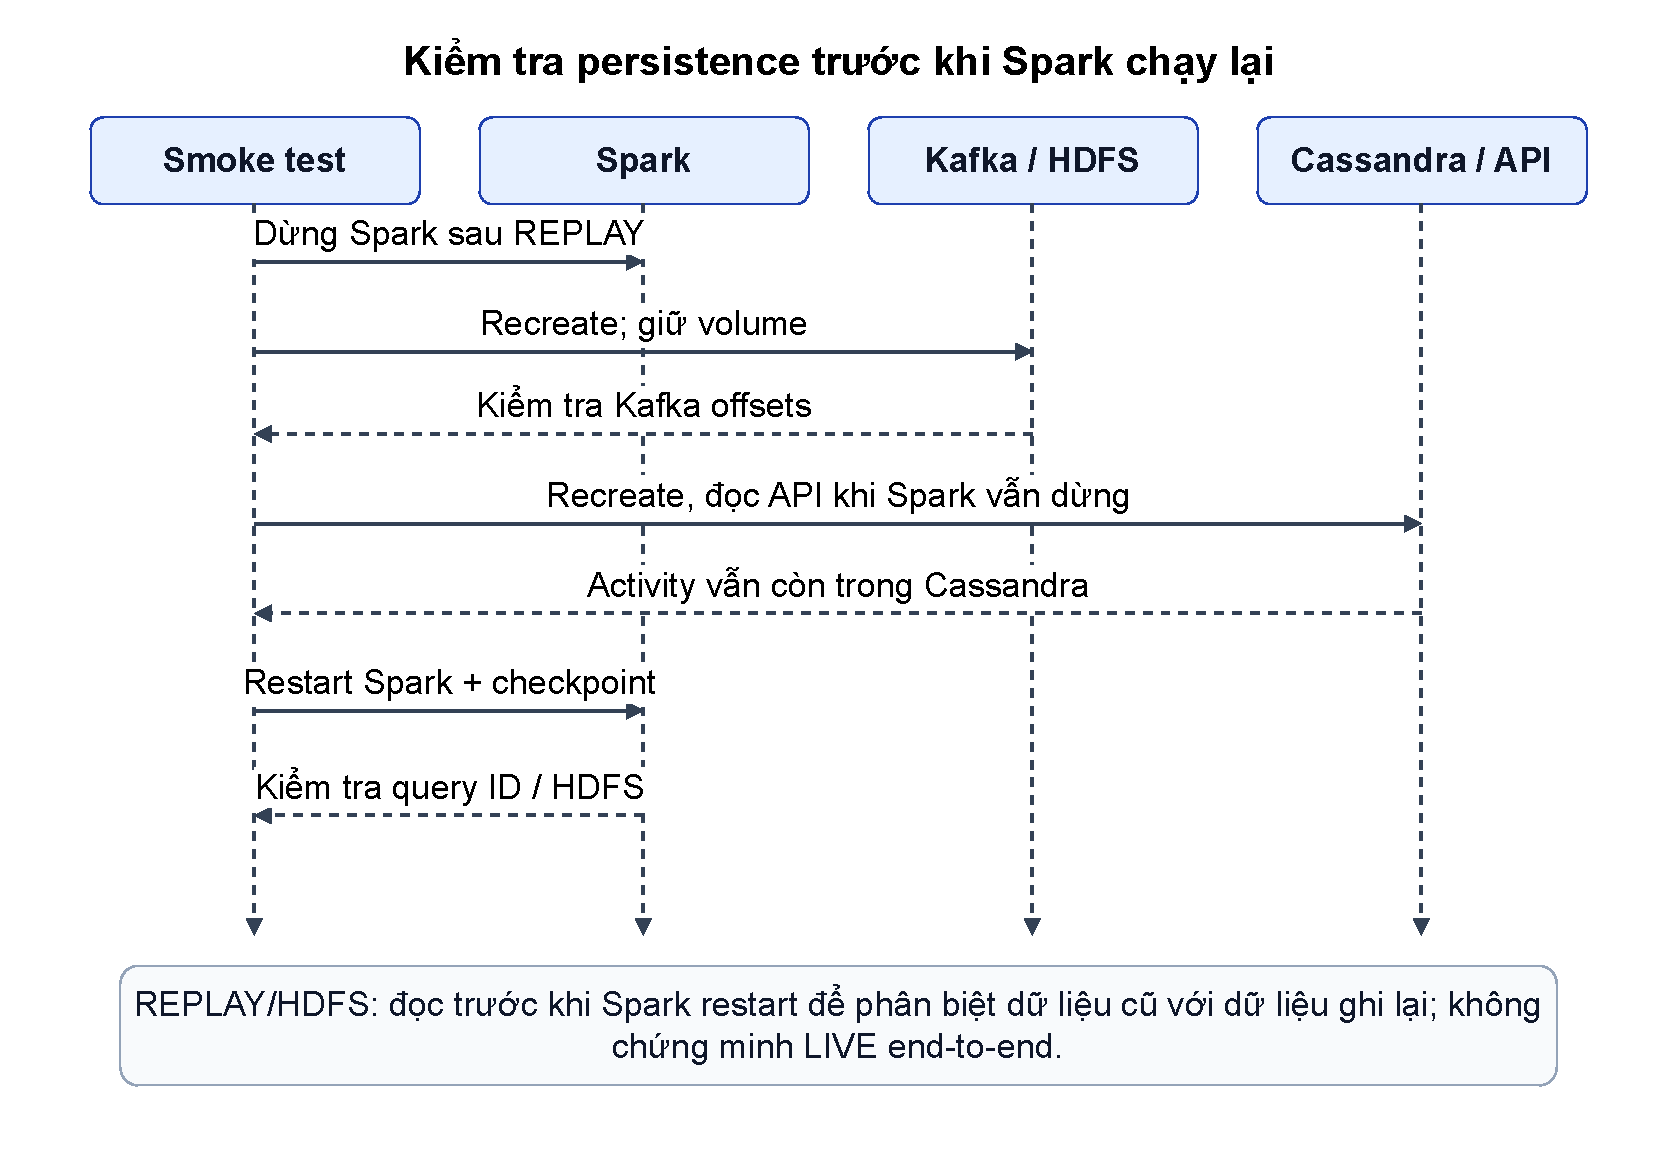
\includegraphics[width=\linewidth]{so-do/seq-recovery.pdf}
\caption{Một kịch bản kiểm thử REPLAY/HDFS: đọc API khi Spark còn dừng giúp kiểm tra dữ liệu Cassandra tồn tại qua restart, trước khi Spark có thể ghi lại.}\label{fig:recovery-sequence}
\end{figure}

Một bài đo W3 khác của Thành gửi 1.200 event tổng hợp dùng cùng key, sau đó khởi động lại Spark. Ba query
\code{bronze\_raw}, \code{bronze\_invalid} và \code{silver\_events} báo input end-offset đạt đích khi được
quan sát ở 8,984 giây sau khi gửi xong; phép đo gồm thời gian khởi động lại và polling. Con số không phải độ trễ
tới API/dashboard, cũng không phải benchmark cho nhiều partition. Nguồn: \code{docs/plans/W3-THANH-01.md}.

\section{Chạy LIVE liên tục}
Ngày 23/11/2026, Thành chạy collector LIVE trong Docker Compose trên Windows trong khoảng 20 phút 45 giây;
collector nhận và ghi nhận ACK liên tiếp cho 40.112 event, với sáu reconnect, không ghi nhận parse error hay
publish failure trong counter. Mạng collector được ngắt có chủ đích 75 giây và số ACK tiếp tục tăng sau khi kết nối lại.
Nguồn: \code{docs/plans/W2-THANH-01.md}.

Cùng ngày, một lượt trên EC2 \code{m7i-flex.large} chạy 30 phút 44 giây. Collector ghi nhận 70.252 event nhận,
70.252 event đã publish, năm reconnect, không restart, \code{parse\_errors=0} và \code{publish\_failed=0}; tổng
Kafka end-offset là 70.252. Counter parse chỉ đếm JSON sai hoặc không phải object, không xác nhận toàn bộ schema.
Sự tương ứng giữa counter và tổng offset không đối chiếu ID duy nhất và không chứng minh không mất/trùng end-to-end.
Smoke REPLAY core trên EC2 đạt tám kiểm tra, không chạy HDFS. Máy dùng snapshot của working tree chưa commit vào
thời điểm thử, không phải clean clone từ commit. Tài nguyên thử đã được dọn. Nguồn:
\code{docs/plans/W4-THANH-01.md}. Các lượt này không tự đóng CP3 hoặc CP4.
\section{Tải và dung lượng}\label{sec:dungluong}
\dukiensua{Tải Spark và latency dưới tải: cần Linh bổ sung evidence.}
\subsection{Dung lượng Cassandra và hạn lưu chi tiết sự kiện}
Số đo lấy trên một node Cassandra 4.1.8 chạy trong Docker trên máy Windows 11. Công cụ đo ghi dữ liệu tổng hợp đúng cấu
trúc contract vào một keyspace tạm, qua cùng lớp truy cập mà Spark dùng. Sau đó công cụ ép Cassandra ghi xuống đĩa, đọc
dung lượng thật, rồi xóa keyspace (Bảng~\ref{tab:dungluong}).

\begin{table}[H]
\centering\small
\caption{Dung lượng và tốc độ ghi đo được}\label{tab:dungluong}
\begin{tabularx}{\linewidth}{@{}Xrrrr@{}}
\toprule
\textbf{Bảng} & \textbf{Dòng} & \textbf{Byte trên đĩa} & \textbf{Byte/dòng} & \textbf{Dòng/giây} \\ \midrule
Chi tiết sự kiện & 20.000 & 2.890.920 & 144,5 & 78 \\
Xu hướng (một cửa sổ) & 5.000 & 84.194 & 16,8 & 79 \\
\bottomrule
\end{tabularx}
\end{table}

Hai dòng của bảng đo hai thứ khác nhau. Dòng đầu là số sự kiện, quyết định hạn lưu. Dòng thứ hai là một cửa sổ xu hướng
đúng bằng giới hạn 5.000 trang, dùng để kiểm tra rằng đọc cả partition lớn nhất được phép vẫn nhanh: lấy top-20 mất
156~ms. Dữ liệu tổng hợp lặp lại nhiều nên nén tốt hơn dữ liệu thật; số byte của bảng xu hướng chỉ để thấy partition
nhỏ, không dùng để ước tính.

Mẫu W1 có khoảng 2,3 event/giây cho hai wiki, tương đương 200.000 event/ngày. Với 145 byte/dòng, ước tính
29~MB/ngày hoặc 200~MB cho 7 ngày; hạn lưu event detail được chọn là 7 ngày. Tốc độ 78 dòng/giây đo trên một node với
fixture tổng hợp không chứng minh khả năng xử lý ổn định tải LIVE toàn cầu.

% ============================================================================
% CHƯƠNG 6: KẾT LUẬN
% ============================================================================

\chapter{Kết luận và hướng phát triển}\label{chap:ketluan}
\setstretch{1.2}
\section{Kết quả đạt được}
WikiPulse kết hợp thu thập thay đổi Wikipedia, xử lý sự kiện theo thời gian, lưu trữ và dashboard để cung cấp thông tin về hoạt động, xu hướng và các chỉnh sửa cần ưu tiên xem xét. Nhóm đã kiểm thử bằng dữ liệu mẫu và nguồn thật trên các môi trường khác nhau; kết quả chi tiết cùng giới hạn của từng phép thử được trình bày trong chương đánh giá.
\section{Hạn chế}
\begin{itemize}
\setlength{\itemsep}{0pt}
\item Cấu hình thử nghiệm dùng một node và chưa có xác thực, phân quyền hay high availability.
\item Cursor chỉ nằm trong bộ nhớ; hệ thống không cam kết không mất hoặc lặp sự kiện hay exactly-once trên toàn bộ luồng.
\item Bronze có thể chứa thông tin cá nhân; thay thế định danh trong Silver không bảo đảm ẩn danh tuyệt đối vì tiêu đề trang vẫn có thể chứa danh tính.
\item Các phép đo và kiểm tra phục hồi chỉ đại diện cho điều kiện đã thử, không phải mọi mức tải hoặc môi trường vận hành.
\end{itemize}
\section{Hướng phát triển}
Các hướng tiếp theo gồm lưu cursor bền vững, mở rộng khả năng phục hồi và bảo mật, đánh giá tải trên dữ liệu đại diện hơn, cải thiện các dấu hiệu ưu tiên và nghiên cứu khả năng triển khai có high availability. Các cải tiến cần được kiểm chứng riêng trước khi áp dụng vào vận hành.
\setstretch{1.5}

\clearpage\phantomsection
\addcontentsline{toc}{chapter}{Tài liệu tham khảo}
\begingroup
\singlespacing
\bibliographystyle{plain}
\bibliography{references}
\endgroup

\end{document}
